\ifnum\switch=1
% -----------------------------------------------------------------------------
% ------------------------------ Extended ToC ---------------------------------
% -----------------------------------------------------------------------------
%data mostly gotten from: PHD_Docs/LaTeX/Shishkin/ETNA17001_revised/Ech.Lie.Szy.Tic.17_rev.tex
Parts of this chapter have already been published in:
\begin{enumerate}
\item[\cite{EchLieSzyTic18}] \underline{C.~Echeverr{\'\i}a}, J.~Liesen, D.~B.~Szyld, and P.~Tich{\'y}, \textbf{Convergence of the multiplicative Schwarz method for singularly perturbed convection-diffusion problems discretized on a Shishkin mesh}, Electron. Trans. Numer. Anal., 48 (2018), pp. 40--62.
\end{enumerate}


\section{Introduction}
This section is based on the following references: \cite{EchLieSzyTic18, GriDolSil15}.
\paragraph{Keywords:}


\section{The Model Problem and its Shishkin Mesh Discretization}
This section is based on the following references: \cite{GriDolSil15}.
\paragraph{Keywords:}


\section{Convergence Bounds for the Multiplicative Schwarz Method}
This section is based on the following references: \cite{EchLieSzyTic18}.
\paragraph{Keywords:}

\subsection{Bounds for the Upwind Difference Scheme}

\subsection{Bounds for the Central Difference Scheme}


\section{The Stagnation of GMRES}
This section is based on the following references: \cite{Gal13, GolVan13, HorJoh12, Saa03}.
\paragraph{Keywords:}


\section{Shishkin-Schwarz Preconditioning}
This section is based on the following references: \cite{KahKamPhi07}.
\paragraph{Keywords:}


\section{Flow-Following Preconditioning}
This section is based on the following references: \cite{ElmSilWat14}.
\paragraph{Keywords:} The name flow following comes from \cite{AndKop96}


\section{Numerical Experiments}
This section is based on the following references: \cite{ElmSilWat14}.
\paragraph{Keywords:}

\subsection{Upwind Finite Differences}
This section is based on the following references: \cite{EchLieSzyTic18, Smi85}.
\paragraph{Keywords:}


\subsection{Central Finite Differences}
This section is based on the following references: \cite{EchLieSzyTic18, Smi85}.
\paragraph{Keywords:}

%\subsection{Preconditioning}



\else
% -----------------------------------------------------------------------------
% --------------------------- Content of Chapter ------------------------------
% -----------------------------------------------------------------------------

Parts of this chapter have already been published in:
\vspace*{0.3cm}
%
\begin{enumerate}
\item[\cite{EchLieSzyTic18}] \underline{C.~Echeverr{\'\i}a}, J.~Liesen, D.~B.~Szyld, and P.~Tich{\'y}, \textbf{Convergence of the multiplicative Schwarz method for singularly perturbed convection-diffusion problems discretized on a Shishkin mesh}, Electron. Trans. Numer. Anal., 48 (2018), pp. 40--62.
\end{enumerate}
%
\vspace*{0.3cm}
%
\section{Introduction}
\label{1D:intro}

In this chapter we study the convergence behavior of both the multiplicative
Schwarz method and the preconditioned GMRES method when they are used to solve
linear systems of the form
%
\begin{equation}\label{eq:1Dlinsys}
\mathscr{A}^{N}u^{N}=\mathscr{F}^{N}
\end{equation}
%
where the coefficient matrix is obtained from both upwind and central finite
difference discretizations of one-dimensional convection-diffusion problem
posed on a Shishkin mesh.

Using the algebraic structure of the iteration matrices, we derive bounds on
the infinity norm of the error produced by the method at each iteration step.
Unlike asymptotic convergence results based on bounding the spectral radius of
the iteration matrix, our results apply to the transient rather than the
asymptotic behavior and thus our error bounds are valid from the first step of
the multiplicative Schwarz iterations.

For linear systems obtained from the upwind scheme we prove rapid convergence
of the  multiplicative Schwarz iteration for all relevant parameters in the
problem. The analysis of the central difference scheme is more complicated,
since some of the submatrices that occur in this case are not only
nonsymmetric, but also fail to be $M$-matrices. This reminds of the analysis
in~\cite{AndKop96}, which showed that in this case the difference scheme
itself does not satisfy a discrete maximum principle. Nevertheless, we can
prove the convergence of the multiplicative Schwarz method for problems
discretized by central differences on a Shishkin mesh under the assumption
that the number of discretization points in each of the local subdomains is
even. If this assumption is not satisfied, then the method may diverge, which
we also explain in our analysis.

Furthermore, we study the convergence of the preconditioned GMRES method when the multiplicatvie Schwarz method is used as a preconditioner and show that the low-rank structure of the iteration matrix $T$ is enough to prove convergence of the preconditioned GMRES method independent of the perturbation parameter $\epsilon$. We also present an analysis of convergence of the method when \emph{Flow-Following} preconditioners are used to precondition the method and show that they are efficient.

The chapter is organized as follows. Section~\ref{1D:Problem} specifies the
model problem and its Shishkin mesh discretization.
%In Section~\ref{s:schwarz} we describe the multiplicative Schwarz method for the discretized problem.
In Section~\ref{1D:GMRESstag} we discuss the performance of GMRES when used to
solve these problems.
In Section~\ref{1D:SchBnds} we present the convergence
analysis of the multiplicative Schwarz method, first for the upwind scheme and
then for the central difference scheme.
In Section~\ref{1D:ShishScwarzPrecon} we discuss the performance of GMRES when preconditioned with multiplicative Schwarz.
In Section~\ref{1D:FlowFollowPrecon} we present an analysis of the convergence of GMRES when a second type of preconditioners is used.
Numerical examples for all cases are shown in Section~\ref{1D:NumericsA}.
% and a concluding discussion, which also puts our results into a broader
% context, is given in Section~\ref{1D:final}.

\section{The Model Problem and its Shishkin Mesh Discretization}
\label{1D:Problem}

We consider the following one-dimensional
convection-diffusion boundary value problem with constant coefficients and
Dirichlet boundary conditions:
\begin{equation}\label{eq:1Dbvp}
\begin{cases}
\mathscr{A}u(x):=
-\epsilon  u''(x) + \omega u'(x)+\beta u(x) = f(x), &  0<x<1,\\
            \qquad\;\;u(0)=u_0,\;\;u(1)=u_1, &
\end{cases}
\end{equation}
%
where $\omega_x\gg \epsilon >0$ and $\beta\geq 0$. We assume that the parameters
of the problem, i.e., $\epsilon,\omega_x,\beta,f,u_0,$ and $u_1$, are chosen
so that the solution $u(x)$ has one boundary layer close to the point $x=1$.
We resolve the boundary layer using a finite difference discretization on a
one-dimensional Shishkin mesh with transition point close to $x=1$ and
consider two different schemes on the mesh: upwind and central differences.

The first derivative of $u$ at the point $x_i$ approximated by the standard
upwind finite difference operator is given by
\begin{equation*}
%\frac{\partial u(x_i)}{\partial x}
u'(x_i)\approx (\Delta x)^{-1}D^{-}_{x} u_{i}^N = (\Delta x)^{-1}(u_{i}^N-u_{i-1}^{N})=\frac{u_i^N-u_{i-1}^{N}}{h_i},
\end{equation*}
and using the central finite difference operator we obtain
\begin{equation*}\label{eq:firstcen}
%\frac{\partial u(x_i)}{\partial x}
u'(x_i)\approx (\Delta x)^{-1} D^{0}_{x} u_{i}^N =(\Delta x)^{-1}(u_{i+1}^N-u_{i-1}^{N})=\frac{u_{i+1}^N-u_{i-1}^{N}}{(h_i+h_{i+1})}.
\end{equation*}
The second derivative can be approximated by
\begin{equation*}
%\frac{\partial u(x_i)}{\partial x^2}
u''(x_i)\approx \delta^{2}_{x} u_{i}^N\; =\;
\frac{2 u_{i-1}^N}{(h_{i} + h_{i+1}) h_{i+1}}- \frac{2u_{i}^N}{h_{i} h_{i+1}} + \frac{2 u_{i+1}^N}{(h_{i} + h_{i+1}) h_{i+1}}.
\end{equation*}
Furthermore, when we apply the discrete operators on the Shishkin mesh where $h_i=h_x$ for $i=1,\ldots,n$ and $h_i=H_{x}$ for $i=n+1,\ldots,M$ (see Figure \ref{fig:back:shmesh1D})we
obtain, for the upwind scheme
\begin{equation}
\Delta^{-}_{x} u_{i}^N\; =\;
\begin{cases}
\frac{1}{H_x}\left(u_{i}^N-u_{i-1}^N\right) & \mbox{for}\;\; i=1,\ldots, n, \\
\frac{1}{h_x}\left(u_{i}^N-u_{i-1}^N\right) & \mbox{for}\;\; i={n+1},\ldots, M,
\end{cases}
\end{equation}
and for the central finite difference operator we obtain
\begin{equation}
\Delta^{0}_{x} u_{i}^N\; =\;
\begin{cases}
\frac{1}{2H_x}\left(u_{i+1}^N-u_{i-1}^N\right) &
\mbox{for}\;\; i=1,\ldots, {n-1},\\
\frac{1}{h_x+H_x}\left(u_{i+1}^N-u_{i-1}^N\right)  &
\mbox{for}\;\; i=n,\\
\frac{1}{2h_x}\left(u_{i+1}^N-u_{i-1}^N\right)  &
\mbox{for}\;\;i={n+1},\ldots, {M}.
\end{cases}
\end{equation}
For the second derivatives, we obtain
\begin{equation}\label{eq:back:second}
\delta^{2}_{x} u_{i}^N\; =\;
\begin{cases}
\frac{1}{H_x^2}\left(u_{i-1}^N - 2u_{i}^N + u_{i+1}^N\right) &
\mbox{for}\;\; i=1,\ldots, {n-1},\\
\frac{2u_{i-1}^N}{(H_x+h_x)H_x} - \frac{2u_{i}^N}{H_xh_x} + \frac{2u_{i+1}^N}{(H_x+h_x)h_x} &
\mbox{for}\;\; i=n,\\
\frac{1}{h_x^2}\left(u_{i-1}^N - 2u_{i}^N + u_{i+1}^N\right) &
\mbox{for}\;\;i={n+1},\ldots, {M}.
\end{cases}
\end{equation}

% Considering the homogeneous boundary conditions $u_0 = u_1 = 0$ and letting
% $\omega(x)=\omega>0$, and $\beta(x) = \beta>0$ be constant along the domain,
% the finite difference scheme applied to the differential equation in \eqref{eq:1Dbvp} on
% the Shishkin mesh is then given~by
% \begin{equation}\label{eq:1DdiscrOp}
% %\mathscr{A}^{N}u^N_m:=
% -\epsilon \delta_x^2 u^N_i + \omega \Delta^{-/0}_{x}u^N_i +\beta_i u^N_i= f_i,\quad i=1,2,\ldots,N-1\equiv M.
% \end{equation}
Thus, by including the boundary conditions and letting
$\omega(x)=\omega>0$ and $\beta(x) = \beta>0$ be constant along the domain,
the finite difference scheme applied to the continuous problem \eqref{eq:1Dbvp} we obtain our model problem:
% consists of the
% following discretization of the one-dimensional convection-diffusion boundary
% value problem with constant coefficients and Dirichlet boundary conditions:
%
\begin{equation}\label{eq:1DbvpD}
\begin{cases}
\mathscr{A}^{N}u^N:=-\epsilon \delta^2 u^N_i + \omega_i \Delta^{-/0}u^N_i +\beta_i u^N_i = f_i, & i=1,\ldots,M,\\
\;\;u^N_0=u_0,\;\;u^N_N=u_1, &
\end{cases}
\end{equation}

By collecting all equations for $i=1,\ldots,M$, both finite difference schemes
yield a linear algebraic system \eqref{eq:1Dlinsys} with the tridiagonal and
nonsymmetric $(N-1)\times (N-1)$ matrix:
%
\begin{equation}\label{eq:back:1Dmatrix}
\mathscr{A}^{N}=\left[
  \begin{array}{cccc|c|cccc}
     \entryvC &\entryvE    &  &  &  &  &  &  &  \\
     \entryvW &\ddots &\ddots  &  &  &  &  &  &  \\
     &  \ddots& \ddots &  \entryvE   &  &  &  &  &  \\
     &  &\entryvW & \entryvC  & \entryvE   &  &  &  &  \\ \hline
     &  &  & \entryzW  & \entryzC  & \entryzE  &  &  &  \\ \hline
     &  &  &  & \entrywW  & \entrywC  & \entrywE  &  &  \\
     &  &  &  &  & \entrywW  & \ddots & \ddots &  \\
     &  &  &  &  &  & \ddots & \ddots & \entrywE  \\
     &  &  &  &  &  &  & \entrywW  & \entrywC  \\
  \end{array}
\right].%\;\in\;{\mathbb R}^{(N-1)\times (N-1)}.
\end{equation}
%
For the upwind scheme, the entries of $\mathscr{A}^{N}$ are given by
%
\begin{align}
    &\entryvW  =  -\frac{\epsilon}{H^{2}} - \frac{\omega_x}{H},&
    &\entryvC  =  \frac{2\epsilon}{H^{2}} + \frac{\omega_x}{H}+\beta, &
    &\entryvE   =  -\frac{\epsilon}{H^{2}}, \nonumber \\
    &\entryzW  =  -\frac{2\epsilon}{H(H+h)} - \frac{\omega_x}{H},&
    &\entryzC  =  \frac{2\epsilon}{hH} + \frac{\omega_x}{H}+\beta,&
    &\entryzE  =  -\frac{2\epsilon}{h(H+h)}, \label{eq:back:upwind} \\
    &\entrywW  =  -\frac{\epsilon}{h^{2}} - \frac{\omega_x}{h},&
    &\entrywC  =  \frac{2\epsilon}{h^{2}} + \frac{\omega_x}{h}+\beta,&
    &\entrywE  =  -\frac{\epsilon}{h^{2}}, \nonumber
\end{align}
%
and for the central difference scheme by
%
\begin{align}
    &\entryvW  =  -\frac{\epsilon}{H^{2}} - \frac{\omega_x}{2H},&
    &\entryvC  =  \frac{2\epsilon}{H^{2}} + \beta, &
    &\entryvE  =  -\frac{\epsilon}{H^{2}}+\frac{\omega_x}{2H}, \nonumber \\
    &\entryzW  =  -\frac{2\epsilon}{H(H+h)} -\frac{\omega_x}{h+H},&
    &\entryzC  =  \frac{2\epsilon}{hH} + \beta,&
    &\entryzE  =  -\frac{2\epsilon}{h(H+h)}+\frac{\omega_x}{h+H}, \label{eq:back:central} \\
    &\entrywW  =  -\frac{\epsilon}{h^{2}} - \frac{\omega_x}{2h},&
    &\entrywC  =  \frac{2\epsilon}{h^{2}} +\beta,&
    &\entrywE  =  -\frac{\epsilon}{h^{2}}+ \frac{\omega_x}{2h}. \nonumber
\end{align}

Moreover, we can express the system matrix \eqref{eq:back:1Dmatrix} using the standard finite difference matrices, see,~\cite[Section~2]{PalSim15}. Consider the following proposition:
%
\begin{prop}
Let $x_i\in\Omega^N=\{x_i\in\overline{\Omega}:i=0,\ldots,N;\},$
be the $N+1$ nodes of the Shishkin mesh. Then the upwind finite
difference discretization of the differential operator in \eqref{eq:1Dbvp}
leads to the following discrete operator:
\begin{equation}\label{eq:1Dkronrep}
A =
A(\epsilon,\omega,\beta, N) =
\epsilon (D_{xx}T+e_{n}v_{y}^T) + \omega_xD_xB_{up/cd} + I,
\end{equation}
where
\begin{eqnarray}
T      &=& \mathrm{tridiag}(1,-2,1) \in \mathbb{R}^{M\times M},\nonumber\\
B_{up} &=& \mathrm{tridiag}(-1,1,0) \in \mathbb{R}^{M\times M},\nonumber\\
B_{cd} &=& \mathrm{tridiag}(-1,1,-1)\in \mathbb{R}^{M\times M},\nonumber\\
D_{x}  &=& \mathrm{diag}\left(\underbrace{H_x^{-1},\dots,
           H_x^{-1}}_{n},\underbrace{h_x^{-1},\ldots,
           h_x^{-1}}_{m}\right)\in\mathbb{R}^{M\times M},\\
D_{xx} &=& \mathrm{diag}\left(\underbrace{-H_x^{-2}, \ldots, -H_x^{-2}}_{m},
           -H_x^{-1}h_x^{-1}, \underbrace{-h_x^{-2},\ldots, -h_x^{-2}}_{m}
           \right)\in\mathbb{R}^{M\times M},\nonumber \\
\omega_x &=& \mathrm{diag}(\omega(x_1),\ldots,
             \omega(x_{N-1}))\in\mathbb{R}^{M\times M},\nonumber \\
v_x  &=& [\underbrace{0,\ldots,0}_{m-1},-\gamma_x,0,\gamma_x,\underbrace{0,\ldots,0}_{m-1}]^T\in\mathbb{R}^{M\times 1},\nonumber
%\quad \gamma_y&=\frac{h_y-H_y}{(H_y+h_y)H_yh_y},\nonumber\\
\end{eqnarray}
with $\gamma_x=\frac{h_x-H_x}{(H_x+h_x)H_xh_x}$ and $e_n$ is the $n$-th
cannonical vector of $\mathbb{R}^{N-1}$.
\end{prop}

\begin{proof}
From\td{this proof is for the 2D case, adapt to the 1D case.} \eqref{eq:back:second} we have that, on the Shishkin mesh, the second derivative in the $x$-direction can be approximated by
\begin{equation*}\label{eq:secondx}
\hspace*{-2em}\delta^{2}_{x} u_{C}\; =\;
\frac{1}{H_x^2}\left[1,-2,1\right]\left[\begin{array}{c} u_W\\u_C\\u_E\end{array}\right] \mbox{for}\;\; i=1,\ldots, K,
\end{equation*}
while the second derivative in the $y$-direction (on the Shishkin mesh) can be approximated by
\begin{equation*}\label{eq:secondy}
\hspace*{-2em}\delta^{2}_{y} u_{C}\; =\;
\begin{cases} \left[u_S,u_C,u_N\right]\frac{1}{H_y^2}\left[\begin{array}{c} 1\\-2\\1\end{array}\right] &\mbox{for}\;\; i=1,\ldots, m, \\
\left[u_S,u_C,u_N\right]\frac{1}{H_yh_y}\left[\begin{array}{c} 1\\-2\\1\end{array}\right] + \left[u_S,u_C,u_N\right]\left[\begin{array}{c}\frac{h_y-H_y}{(H_y+h_y)H_yh_y} \\0\\\frac{H_y-h_y}{(H_y+h_y)H_yh_y}\end{array}\right] &\mbox{for}\;\; i=n,\\
\left[u_S,u_C,u_N\right]\frac{1}{h_y^2}\left[\begin{array}{c} 1\\-2\\1\end{array}\right] &\mbox{for}\;\; i=n+1,\ldots, M.\end{cases}
\end{equation*}
Collecting these relations for all rows $i$ and for all columns $j$ for the whole domain we obtain
\[
-\frac{\partial^2 u(x_i,y_j)}{\partial x^2}\approx D_{xx}TU,\quad -\frac{\partial^2 u(x_i,y_j)}{\partial y^2}\approx U(D_{yy}T+v_ye_n^T),
\]
with $D_{xx}$, $D_{yy}$, $v_x$ and $v_y$ defined as above.  The matrix $T$ represents the unscaled approximations to the second derivative in one dimension. The matrices $D_{xx}$ and $D_{yy}$ are the scaling matrices which account for the different mesh sizes of the hybrid mesh in each direction. The term $e_nv_y^T$ is a rank-one operator which, when added to the scaled matrix, accounts for the uneven factor which multiplies the middle point $y_n$ in the $y$-direction of the mesh. With these approximations we can write the following classical matrix formulation of the finite difference discretization of the Poisson equation on a square domain discretized by a hybrid mesh
\begin{equation}\label{eq:PoissonMatrix}
D_{xx}TU+ U(D_{yy}T+v_ye_n^T)=F,\quad\text{where}\quad F_{i,j}=f(x_i,y_j) + \text{b.c.}
\end{equation}
We can now reshape this matrix equation to obtain its Kronecker formulation; see \cite[Section 1.3.7]{GolVan13}. We know that for a matrix equation $Y=CXB$, where $X$ is the matrix of unknowns, it holds that
\[ \text{vec}(Y)=\text{vec}(CXB)=(B^T\otimes C)\text{vec}(X).\]
By applying this result to \eqref{eq:PoissonMatrix} we obtain the following formulation,
 \begin{equation}\label{eq:PoissonKron}
 (I_M\otimes T_x + T_y\otimes I_M+e_nv_y^T \otimes I_M)\text{vec}(U)=\text{vec}(F),
 \end{equation}
 with $T_x=D_{xx}T$, and $T_y=D_{yy}T$. Thus, the discrete Laplacian on the hybrid mesh is
 \begin{equation}\label{eq:PoissonKron}
I_M\otimes T_x +(T_y+ e_nv_y^T) \otimes I_M.
 \end{equation}
It remains to show the Kronecker structure of the first order term of \eqref{eq:bvp}.

When we assume separable convection coefficients, we have
\begin{align*}
\omega_x \cdot \nabla u &=(\phi_1(x_i)\psi_1(y_j),\phi_2(x_i),\psi_2(y_j))\cdot\left( \frac{\partial u(x_i,y_j)}{\partial x},\frac{\partial u(x_i,y_j)}{\partial y}\right)\\
&\approx \phi_1(x_i)\psi_1(y_j)D^{-}_{x} u_{C} + \phi_2(x_i)\psi_2(y_j)D^{-}_{y} u_{C}.
\end{align*}
 We can approximate these terms by using \eqref{eq:firstup}; for the $x$-direction we obtain
\begin{equation*}
\phi_1(x_i)\psi_1(y_j)D^{-}_{x} u_{C}\; =\;
\frac{1}{H_x}\phi_1(x_i)\left[-1,1,0\right]\left[\begin{array}{c} u_W\\u_C\\u_E\end{array}\right]\psi_1(y_j) \mbox{for}\;\; i=1,\ldots, K.
\end{equation*}
For the $y$-direction (from the right) we obtain
\begin{equation*}
\hspace*{-1em}\phi_2(x_i)\psi_2(y_j)D^{-}_{y} u_{C}\; =\;
\begin{cases} \phi_2(x_i)\frac{1}{H_y}\left[u_S,u_C,u_N\right]\left[\begin{array}{c} -1\\1\\0\end{array}\right]\psi_2(y_j) &\mbox{for}\;\; i=1,\ldots, n, \\
 \phi_2(x_i)\frac{1}{h_y}\left[u_S,u_C,u_N\right]\left[\begin{array}{c} -1\\1\\0\end{array}\right]\psi_2(y_j)&\mbox{for}\;\; i=n+1,\ldots, M.\end{cases}
\end{equation*}
Collecting these results for all grid nodes and recalling that $u_C$ is the approximation of $u$ at the point $(x_i,y_j)$, we obtain
\begin{eqnarray*}
\left(\phi_1(x_i)\psi_1(y_j)\frac{\partial u(x_i,y_j)}{\partial x}\right)_{i,j=0,\ldots,J}\approx\Phi_{1}(D_xBU)\Psi_{1},\\
\left(\phi_2(x_i)\psi_2(y_j)\frac{\partial u(x_i,y_j)}{\partial y}\right)_{i,j=0,\ldots,N}\approx\Phi_{2}U(D_yB)^T\Psi_{2}.
\end{eqnarray*}
Thus \eqref{eq:bvp} has the following matrix equation representation
\begin{equation*}
\epsilon D_{xx}TU + \epsilon U(D_{yy}T+e_nv_y^T) +\Phi_{1}(D_xB)U\Psi_{1}+\Phi_{2}U(D_yB)^T\Psi_{2}=F,
\end{equation*}
or, equivalently, by applying \cite[Lemma~6.5]{Dem97} we obtain its Kronecker formulation:
\[
\hspace*{-2em}
 \left[\epsilon \left(I_M\otimes T_x\right) +\epsilon\left(T_y\otimes I_M+t_y \otimes I_M\right) + \Psi_1 \otimes \Phi_1B_{x} + \Psi_2B_{y} \otimes \Phi_2\right]\text{vec}(U) =\text{vec}(F).
\]
Thus we have shown that the discrete operator takes the desired form \eqref{eq:kronrep}.
\end{proof}


If $u_{h}=A_{h}^{-1}f_{h}=[u_1^N,\dots,u_{N-1}^N]^T$ is the exact algebraic
solution, and $u(x)$ is the solution of \eqref{eq:1Dbvp}, then there exist constants $c_1,c_2>0$ such that
%
$$\max_{1\leq i\leq N-1}\,|u(x_i)-u_i^N| \leq c_1 \frac{\ln N}{N}$$
%
for the upwind scheme, and
%
$$\max_{1\leq i\leq N-1}\,|u(x_i)-u_i^N| \leq c_2 \left(\frac{\ln N}{N}\right)^2$$
%
for the central difference scheme. Thus, the convergence of both schemes is
$\epsilon$-uniform, and the central difference scheme is more accurate than the
upwind scheme. As pointed out by Stynes~\cite[p.~470]{Sty05}, the convergence
proof for the central differences (originally due to Andreyev and
Kopteva~\cite{AndKop96}) is complicated since the scheme does not satisfy a
discrete maximum principle. We meet similar complications in our analysis in
Section~\ref{ss:central} below.
%
Both schemes lead to highly ill-conditioned matrices $A$. The main reason is
the large difference between the mesh sizes $H$ and $h$, which implies large
differences between the moduli of the nonzero entries of $A$ corresponding to
each subdomain. Thus, $A$ is poorly scaled. As shown by Roos~\cite{Roo96}, a
simple diagonal scaling reduces the order of the condition number for the
matrix from the upwind scheme from $\mathscr{O}(\epsilon^{-1}(N/\ln N)^2)$ to
$\mathscr{O}(N^2/\ln N)$. Although not shown by Roos, an analogous diagonal
scaling appears to work well also for the central difference scheme; see
Section~\ref{ss:scaling} for the exact form of the scaling matrices. The first
row in the following table shows a numerical illustration for
$\epsilon=10^{-8}$, $\omega_x=1$, $\beta=0$ in \eqref{eq:1Dbvp}, and $N=198$.

\begin{table}[h!]\centering
\begin{tabular}{r|c c c c}
&upwind & upwind scaled & central & central scaled\\
\hline
matrix cond. & $4.0500 \times 10^{10}$ & $2.9569\times 10^{3}$ &
$6.2323 \times 10^{10}$ & $2.9514 \times 10^{3}$\\
eigenvector cond. & $1.5143 \times 10^{17}$ & $1.2297 \times 10^{19}$ &
$4.1070\times 10^{3}$ & $1.8682\times 10^{2}$
\end{tabular}
\end{table}

The second row of the table shows the condition numbers of the eigenvector
matrices from the decomposition $A=VDV^{-1}$ computed by {\tt [V,D]=eig(A)} in
MATLAB. We observe that the upwind scheme yields matrices with very ill-
conditioned eigenvectors, i.e., highly nonnormal matrices. Apparently, the
eigenvector conditioning is not much affected by the diagonal scaling.


\section{Convergence Bounds for the Multiplicative Schwarz Method}\label{1D:SchBnds}

We stuy the convergence of the multiplicative Schwarz method applied to upwind
and central finite difference discretizations of one-dimensional singularly
perturbed convection-diffusion model problems posed on a Shishkin mesh. The
matrices that arise from the discretization are nonsymmetric, and usually
nonnormal as well as ill-conditioned,which leads to very slow convergence of
standard iterative solvers like the (unpreconditioned) GMRES method.

In the simple one-dimensional case analyzed in this paper, the Shishkin mesh
divides the discretized domain into two local subdomains where the solution
presents a different characteristic nature. Therefore, a solution approach
based on domain decomposition methods seemed only natural. For the upwind
scheme, we proved rapid convergence of the multiplicative Schwarz method for
all relevant problem parameters. The convergence for the central difference
scheme is slower, but still rapid, when $N^2\epsilon < \omega_x$ and if $N/2-1$
is even.


We start with a closer look at the structure of the iteration matrix $T$.
Note that the matrices $P_i$ from \eqref{eq:Pi} satisfy
%
\begin{align*}
P_1 &= R_1^TA_1^{-1}R_1A
=\left[\begin{array}{c} I_{n}\\ 0\end{array}\right]\matAs_1^{-1}
\left[\begin{array}{c|c|c}\matAs_1 & \entryzE e_n & 0\end{array}\right]=
\left[\begin{array}{c|c|c}I_{n}&\entryzE \matAs_1^{-1}e_{n}&0\\\hline 0&0&0\end{array}\right],
\end{align*}
%
and
%
$$P_2 = R_2^TA_2^{-1}R_2A =
\left[\begin{array}{c} 0 \\  I_n\end{array}\right] A_2^{-1}
\left[\begin{array}{c|c|c}0 & \entryzW e_1 & \matAs_2 \end{array}\right]=
\left[\begin{array}{c|c|c}0&0&0\\\hline0&\entryzW \matAs_2^{-1}e_1&I_{n}\end{array}\right],$$
%
\cred{where $e_1$, $e_n\in \mathbb{R}^n$.} We now denote
%
\begin{equation}\label{eq:1D:p_and_pi}
\left[\begin{array}{c}\pOne \\\hline \piOne\end{array}\right]
\equiv \entryzE\matAs_1^{-1}e_n\quad\mbox{and}\quad
\left[\begin{array}{c} \piTwo\\\hline \pTwo\end{array}\right]
\equiv \entryzW\matAs_2^{-1}e_1,
\end{equation}
%
where $\pI=[\pI_1,\dots,\pI_m]^T\in{\mathbb R}^m$ for $i=1,2$, and $\piOne$
and $\piTwo$ are scalars. Then
%
$$I - P_2  =
\left[\begin{array}{c|c|c}I_{m-1}&0&0\\\hline
0&1&0\\\hline 0&-\left[\begin{array}{c} \piTwo\\\hline \pTwo\end{array}\right]&0\end{array}\right],\qquad
I - P_1  =
\left[\begin{array}{c|c|c}0&-\left[\begin{array}{c}\pOne \\\hline \piOne\end{array}\right]&0\\\hline 0&1&0\\\hline 0&0&I_{m-1}\end{array}\right],$$
%
which gives
%
\begin{equation}\label{eq:1D:struct1}
(I-P_2)(I-P_1) = \left[\begin{array}{c|c|c}0&-\pOne&0\\\hline 0&\pOne_m\piTwo&0\\\hline 0&\pOne_m \pTwo&0\end{array}\right]=
\left[\begin{array}{c}-\pOne\\\hline \pOne_m\piTwo\\\hline \pOne_m \pTwo\end{array}\right]
e_{n+1}^T,
\end{equation}
%
and
%
\begin{equation}\label{eq:1D:struct2}
(I-P_1)(I-P_2)=
\left[\begin{array}{c}
 \pTwo_1 \pOne\\
\hline
 \pTwo_1\piOne\\
 \hline
  -\pTwo\end{array}\right]
e_{n-1}^T,
\end{equation}
\cred{where $e_{n+1}$, $e_{n-1}\in \mathbb{R}^{N-1}$}.
%
Thus, both iteration matrices have rank one, and we
can apply to them the following observation.

\begin{prop} \label{thm:1D:rank.one}
Let $T$ be a square matrix of rank one, i.e., $T=uv^T$ for some
vectors $u, v$. Then $T^2 = \rho T$, with $\rho = v^Tu$, and as
a consequence $T^{k+1} = \rho^{k} T$, for $k\geq 0$.
\end{prop}

\begin{proof}
The proof follows by direct computation.
\end{proof}

\begin{cor}
In the notation established above, let $T=(I-P_2)(I-P_1)$ or
$T=(I-P_1)(I-P_2)$. Then for any $k\geq 0$ we have
%
\begin{equation}\label{eq:Tkp1}
T^{k+1} =  \rho^{k} T,\quad\mbox{where}\quad \rho \equiv \pOne_m \pTwo_1.
\end{equation}
%
\end{cor}

\begin{proof}
Applying Proposition~\ref{thm:1D:rank.one} to either
\eqref{eq:1D:struct1} or \eqref{eq:1D:struct2} produces the desired result.
%
\end{proof}

Equation \eqref{eq:Tkp1} shows, in particular, that
$\|T^{k+1}\|=|\rho|^k \|T\|$ holds for any matrix norm $\|\cdot\|$.
In order to obtain a convergence bound for the multiplicative Schwarz method
we will bound $|\rho|$ and $\|T\|_\infty$. The following lemma will be
essential in our derivations.

\begin{lemma} \label{lem:pp}
In the notation established above,
%
$$\left[\begin{array}{c}\pOne \\\hline \piOne\end{array}\right]
= \piOne \left[\begin{array}{c}-\entryvE \matAH^{-1}e_{m } \\
\hline 1\end{array}\right],\qquad
\piOne=\frac{\entryzE }{\entryzC -\entryzW \entryvE  \left(\matAH ^{-1}\right)_{m,m}},$$
%
$$\left[\begin{array}{c} \piTwo\\\hline \pTwo\end{array}\right]=
\piTwo \left[\begin{array}{c}1 \\
\hline -\entrywW\matAh ^{-1}e_1\end{array}\right],\qquad
\piTwo=\frac{\entryzW }{\entryzC - \entryzE \entrywW \left(\matAh ^{-1}\right)_{1,1}}.$$
%
\end{lemma}

\begin{proof}
From \eqref{eq:1D:p_and_pi} we know that $\pOne$, $\pTwo$, $\piOne$, and $\piTwo$
solve the %(saddle point)
systems
%
\begin{equation*}%\label{eq:spp}
\left[\begin{array}{c|c}\matAH &\entryvE  e_{m }\\\hline \entryzW e_{m }^T&\entryzC  \end{array}\right]
\left[\begin{array}{c}\pOne \\\hline \piOne\end{array}\right]
=\entryzE e_n,\qquad
\left[\begin{array}{c|c}\entryzC &\entryzE  e_{1}^T\\\hline \entrywW e_{1}&  \matAh\end{array}\right]
\left[\begin{array}{c}\piTwo \\\hline \pTwo\end{array}\right]
=\entryzW e_1.
\end{equation*}
%
Hence the expressions for  $\pOne$, $\pTwo$, $\piOne$, and $\piTwo$ can be
obtained using Schur complements.
\end{proof}

\cred{Combining \eqref{eq:Tkp1} and Lemma~\ref{lem:pp} gives
%
\begin{equation}\label{eq:1D:rho}
\rho = \frac{\entryzE\, \entryvE  \left(\matAH ^{-1}\right)_{m,m} }{\entryzC -\entryzW\, \entryvE  \left(\matAH ^{-1}\right)_{m,m}}\cdot\frac{\entryzW\, \entrywW \left(\matAh ^{-1}\right)_{1,1}}{\entryzC - \entryzE\, \entrywW \left(\matAh ^{-1}\right)_{1,1}}.
\end{equation}
%
In order to bound $|\rho|$ we thus need to bound certain entries of inverses
of the tridiagonal Toeplitz matrices $\matAH$ and $\matAh$. Lemma ??\td{add label to lemma in the introduction} shows that this is straightforward in the case of an $M$-matrix. As we
will see later in Lemma~\ref{lem:1D:bounds} and Lemma~\ref{lem:1D:p2}, the matrix
$\matAh$ is an $M$-matrix for both the upwind and the central difference
scheme. However, while $\matAH$ is an $M$-matrix for the upwind scheme, it is
not an $M$-matrix in the most common situation for the central
difference scheme. We then have to use a different technique for bounding the
entry $(\matAH^{-1})_{1,1}$; see Section~\ref{ss:central}.}

\noindent
In the next two subsubsections we separately treat the upwind and the central
difference schemes.

\subsection{Bounds for the Upwind Difference Scheme}
\label{1D:SchBnds:upwind}

Using Lemma~\ref{lem:App:MMat} we can prove the following result for the upwind
scheme.

\begin{lemma}\label{lem:1D:bounds}
For the upwind scheme both matrices $\matAH$ and $\matAh$ satisfy the
assumptions of Lemma~\ref{lem:App:MMat}, and the related quantities from
Lemma~\ref{lem:pp} satisfy
%
$$|\piOne|\leq 1, \quad \|\pOne\|_\infty =|\pOne_m|\leq \frac{\epsilon}{\epsilon+\omega_x H},
\quad |\piTwo|\leq 1,\quad \|\pTwo\|_\infty=|\pTwo_1|\leq 1.$$
%
\end{lemma}

{\em Proof.}
%\begin{proof}
It is easy to see from \eqref{eq:back:upwind} that both matrices $\matAH$ and
$\matAh$ resulting from the upwind scheme satisfy the assumptions of
Lemma~\ref{lem:App:MMat}. Thus, from \eqref{eq:min_cond} we have
%
$$|\entryvE| \left(\matAH ^{-1}\right)_{m,m} \leq 1 \quad\mbox{and}\quad
|\entrywW| \left(\matAh ^{-1}\right)_{1,1} \leq 1.$$
%
Moreover, $\entryzC>0$ and $\entryzE,\entryzW<0$, as well as
$\entryzC+\entryzE+\entryzW=\beta \geq 0$, so that
%
\begin{align*}
|\piOne|&=\frac{|\entryzE| }{\entryzC +\entryzW |\entryvE|  \left(\matAH ^{-1}\right)_{m,m}}
\leq\frac{|\entryzE| }{\entryzC + \entryzW}\leq 1,\\
|\piTwo|&=\frac{|\entryzW| }{\entryzC + \entryzE |\entrywW| \left(\matAh ^{-1}\right)_{1,1}}\leq
\frac{|\entryzW| }{\entryzC + \entryzE}\leq 1.
\end{align*}
%
Using these inequalities and the fact that the entries of $\matAh$ decay along
a column away from the diagonal yields
%
$$\|\pTwo\|_\infty=|\pTwo_1|=|\piTwo|\,|\entrywW| \left(\matAh ^{-1}\right)_{1,1}\leq 1.$$
%
Using the decay of the entries of $\matAH$ and
%
$$|\entryvE|  \left(\matAH ^{-1}\right)_{m,m} \leq \left|\frac{\entryvE}{\entryvW}\right|,$$
%
which follows from \eqref{eq:min_cond}, as well as the definitions of the
entries in \eqref{eq:back:upwind}, we obtain
%
$$\|\pOne\|_\infty = |\pOne_m| = |\piOne|\,|\entryvE|
\left(\matAH ^{-1}\right)_{m,m}
\leq \left|\frac{\entryvE}{\entryvW}\right| =
\frac{\epsilon}{\epsilon+\omega_x H%\frac{2\omega_x}{N}
}. ~~ \qed
$$
%
%\cblue{where the last inequality follows from $\frac{2}{N}=H+h\leq 2H$.}
%%\end{proof}

We can now state our main result of this subsection.

\begin{thm} \label{thm:1D:upwind_conv}
For the upwind scheme we have
%
\begin{equation}\label{eq:1D:bound_upw}
|\rho| \leq \frac{\epsilon}{\epsilon+\omega_x H}
%\footnote{\cred{the case $\omega_x=0$ is not considered.}},
\end{equation}
%
and
%
\begin{align*}
\| (I-P_2)(I-P_1) \|_\infty \leq \frac{\epsilon}{\epsilon+\omega_x H},\qquad
\| (I-P_1)(I-P_2) \|_\infty \leq 1.
\end{align*}
%
Thus, the error of the multiplicative Schwarz method \eqref{eq:schwarz}
satisfies
%
$$\frac{\|e^{(k+1)}\|_\infty}{\|e^{(0)}\|_\infty} \leq
\begin{cases} \left( \frac{\epsilon}{\epsilon+\omega_x H}\right)^{k+1}, &\mbox{if}\;\; T=(I-P_2)(I-P_1), \\
\left( \frac{\epsilon}{\epsilon+\omega_x H}\right)^{k}, &\mbox{if}\;\; T=(I-P_1)(I-P_2). \end{cases}$$
%
\end{thm}

\begin{proof}
For the bound on $|\rho|$ we apply Lemma~\ref{lem:1D:bounds} to the expression
$\rho=\pOne_m \pTwo_1$ from \eqref{eq:Tkp1}.
%
From \eqref{eq:1D:struct1} and \eqref{eq:1D:struct2} we respectively see that
%
\begin{align*}
\|(I-P_2)(I-P_1)\|_\infty &= \left\|\left[\begin{array}{c}
-\pOne\\
\hline
\pOne_m\piTwo\\
\hline
\pOne_m \pTwo
\end{array}\right]\right\|_\infty
\quad\mbox{and} \\
\|(I-P_1)(I-P_2)\|_\infty &= \left\|\left[\begin{array}{c}
\pTwo_1 \pOne\\
\hline
\pTwo_1\piOne\\
\hline
-\pTwo\end{array}\right]\right\|_\infty.
\end{align*}
%
Thus, using Lemma~\ref{lem:1D:bounds},
%
\begin{align*}
\| (I-P_2)(I-P_1) \|_\infty &= \max\left\{|\pOne_m|, \ |\pOne_m \piTwo|,\ |\pOne_m \pTwo_1|\right\} \leq |\pOne_m|\leq \frac{\epsilon}{\epsilon+\omega_x H},\\
\| (I-P_1)(I-P_2) \|_\infty &= \max\left\{|\pTwo_1 \pOne_m|, \ |\pTwo_1 \piOne|,\ | \pTwo_1|\right\}
\leq | \pTwo_1|\leq 1.
\end{align*}
%
Using these bounds and \eqref{eq:Tkp1} in the first inequality in
\eqref{eq:error} yields the convergence bound for the multiplicative Schwarz
method.
\end{proof}

Suppose that $\epsilon < \omega_x H$, which is a reasonable assumption in our
context. Then
%
$$|\rho|=\frac{\epsilon}{\epsilon+\omega_x H} = \frac{\epsilon}{\omega_x H}
+ \mathscr{O}\left(\left(\frac{\epsilon}{\omega_x H}\right)^2\right).$$
%
This expression shows that the convergence of the multiplicative Schwarz
method in case of the upwind scheme and a strong convection-dominance will be
very rapid. Numerical examples are shown in Section~\ref{s:numerics}.

Note that since $\frac{2}{N} = H+h \leq 2H$, we have $\frac{1}{N} \leq H$,
\cred{and hence
\begin{equation}\label{eq:1D:bb}
|\rho|\leq \frac{\epsilon}{\epsilon + \omega_x H} \leq \frac{\epsilon}{\epsilon + \frac{\omega_x}{N}}.
\end{equation}
Using the expression on the right hand of (\ref{eq:1D:bb}) in
Theorem~\ref{thm:1D:upwind_conv} would give (slightly) weaker convergence bounds
for the multiplicative Schwarz method. However, the right hand side of
(\ref{eq:1D:bb}) represents a more convenient bound on the convergence factor
which directly depends on the parameters $\epsilon$, $\omega_x$ and $N$ of our
problem.}

\subsection{Bounds for the Central Difference Scheme}
\label{1D:SchBnds:central}

We will now consider the discretization by the central difference scheme,
i.e., the matrix $A$ with the entries given by \eqref{eq:back:central}. It turns
out that the analysis for this scheme is more complicated than for the upwind
scheme since, \cred{as mentioned above, the matrix $\matAH$ need not be an $M$-
matrix. Moreover, as we will see below, the multiplicative Schwarz method may
not converge when the parameter $m$ is odd.}


%\cblue{Moreover, we have numerically observed that if $m$ is even,
%then the multiplicative Schwarz method always converges, while
%for odd $m$, it can diverge. Indeed, for the most common situation $\omega_x H >  2\epsilon$, the %analysis presented in this section shows
%that if $m$ is even, then one can use a technique based on results by Usmani \cite{Usm94} to %bound the term
%\begin{equation}\label{eq:critical}
%\entryvE  \left(\matAH ^{-1}\right)_{m,m},
%\end{equation}
%which represents a critical part of the convergence factor \eqref{eq:1D:rho},
%by a number strictly less than one. On the other hand, if $m$ is odd, then \eqref{eq:critical} %can be greater than one; see Lemma~\ref{lem:1D:usmani} and the corresponding discussion.
%}

The following result about the entries $\entryzC$, $\entryzE$, and $\entryzW$
of $A$ will be frequently used below.


\begin{lemma}
For the central difference scheme we have
%
\begin{equation}\label{eq:1D:bc}
\entryzC>0,\quad \entryzW, \entryzE<0,\quad
-(\entryzW+\entryzE)=|\entryzW|+|\entryzE|
= \entryzC-\beta \leq\entryzC\quad \mbox{and}\quad
\left|\frac{\entryzE}{\entryzC}\right|<1.
\end{equation}
%
\end{lemma}

{\em Proof.}
%\begin{proof}
The inequalities $\entryzC>0$ and $\entryzW<0$ are obvious from
\eqref{eq:back:central}. From \eqref{eq:tau}--\eqref{eq:epsi} we have, since
$N\geq 4$,
%
\begin{equation}\label{eq:1D:alpha_ineq}
\omega_x h = 2\epsilon \,\frac{2\ln N}{N} < 2\epsilon,
\end{equation}
%
and therefore
%
$$\entryzE=\frac{\omega_x h-2\epsilon}{h(H+h)}<0.$$
%
Moreover, $-(\entryzW+\entryzE)=\entryzC -\beta \leq a$, which yields
%
\begin{eqnarray*}
\left|\frac{\entryzE}{\entryzC}\right|  =
\left|\frac{\entryzE}{\beta-(\entryzW+\entryzE)}\right|<1. ~~ \qed
\end{eqnarray*}
%
%\end{proof}

We next consider the matrix $\matAh$ from the central difference scheme.

\begin{lemma}\label{lem:1D:p2}
The matrix $\matAh$ from the central difference scheme satisfies the
assumptions of Lemma~\ref{lem:App:MMat}, and for the corresponding quantities from
Lemma~\ref{lem:pp} we have
%
$$\left|\piTwo\right|\leq 1 \quad\mbox{and}\quad
\|\pTwo\|_\infty=\left|\pTwo_{1}\right|\leq 1.$$
\end{lemma}

\begin{proof}
The inequalities $\entrywC>0$ and $\entrywW<0$ are obvious from
\eqref{eq:back:central}, and using \eqref{eq:1D:alpha_ineq} we obtain
%
$$\entrywE=\frac{\omega_x h-2\epsilon}{2h^{2}}<0.$$
%
Since also
%
$$|\entrywW|+|\entrywE|=\frac{2\epsilon}{h^{2}}\leq\entrywC,$$
%
the matrix $\matAh$ satisfies the assumptions of Lemma~\ref{lem:App:MMat}. Thus,
in particular, $|\entrywW| \left(\matAh ^{-1}\right)_{1,1}\leq 1$.
Using also \eqref{eq:1D:bc} gives
%
$$|\piTwo|=\frac{|\entryzW| }{\entryzC + \entryzE |\entrywW|
\left(\matAh ^{-1}\right)_{1,1}}\leq
\frac{|\entryzW| }{\entryzC + \entryzE}
= \frac{|\entryzW| }{|\entryzW|+\beta}\leq 1.$$
%
Finally, since the entries of $\matAh$ decay along a column away from the
diagonal, we obtain
%
$\|\pTwo\|_\infty=
\left|\pTwo_{1}\right|=|\piTwo|\,|\entrywW| \left(\matAh ^{-1}\right)_{1,1}
\leq 1$.
%
\end{proof}

We now concentrate on bounding the quantities from Lemma~\ref{lem:pp} related
to the matrix $\matAH$ for the central difference scheme. We will distinguish
\cred{the three cases $\omega_x H<2\epsilon$, $\omega_x H=2\epsilon$, and $\omega_x
H>2\epsilon$ or, equivalently, the cases that the entry
%
$$\entryvE=\frac{\omega_x H-2\epsilon}{2H^{2}}$$
%
of $A_H$ is negative, zero, or positive. It is clear from \eqref{eq:1D:rho} that
the sign of $b_H$ is important for the value $|\rho|$.}

A simple computation shows that $\entryvE\leq 0$ if and only if
%
$$\epsilon \geq \frac{\omega_x}{N+2\ln N} ~\cdot$$
%
If $\epsilon \ll \omega_x\approx 1$, then this condition means that
$\epsilon (N+2\ln N) = \mathscr{O}(1)$, which is an
unrealistic assumption on the discretization parameter $N$. Nevertheless, we
\cred{include the case $b_H\leq 0$ for completeness.}

We first assume that
%
\begin{equation}
\omega_x H<2\epsilon,\label{eq:1D:AHMmatrix}
\end{equation}
%
which means that $\entryvE<0$.
%
\begin{lemma}\label{lem:1D:p3}
If \eqref{eq:1D:AHMmatrix} holds, then the matrix $\matAH$ from the central
difference scheme satisfies the assumptions of Lemma~\ref{lem:App:MMat}, and we have
%
\begin{equation*}%\label{eq:boundC}
\left|\piOne\right|\leq 1 \quad\mbox{and}\quad
\left\Vert\pOne\right\Vert_\infty=\left|\pOne_{m}\right|
<\frac{\epsilon}{\epsilon+\frac{\omega_x}{N}}.
\end{equation*}
\end{lemma}


\begin{proof}
The inequalities $\entryvC>0$ and $\entryvW<0$ are obvious from
\eqref{eq:back:central}, and $\entryvE<0$ holds because of \eqref{eq:1D:AHMmatrix}.
Moreover,
%
$$|\entryvW|+|\entryvE|=\frac{\omega_x}{2H}+\frac{\epsilon}{H^{2}}+
\frac{\epsilon}{H^{2}}-\frac{\omega_x}{2H}=\frac{2\epsilon}{H^{2}}\leq\entryvC,$$
%
so that the matrix $\matAH$ satisfies the assumptions of Lemma~\ref{lem:App:MMat}.
In particular,
%
$$|\entryvE|  \left(\matAH ^{-1}\right)_{m,m}\leq 1.$$
%
Using~\eqref{eq:1D:bc} we obtain
%
$$|\piOne|=\frac{|\entryzE| }{\entryzC +\entryzW |\entryvE|
\left(\matAH ^{-1}\right)_{m,m}}
\leq\frac{|\entryzE| }{\entryzC + \entryzW}\leq 1.$$

Moreover, using that the entries of $\matAH$ decay along a column away from
the diagonal as well as
%
$$|\entryvE|  \left(\matAH ^{-1}\right)_{m,m}\leq
\frac{|\entryvE|}{|\entryvW|},$$
%
which follows from \eqref{eq:min_cond}, we see that
%
\begin{align*}
\left\Vert\pOne\right\Vert_\infty & =\left|\pOne_{m}\right| = |\piOne|\,
|\entryvE|  \left(\matAH ^{-1}\right)_{m,m}\leq
\frac{|\entryvW|}{|\entryvE|} =\frac{2\epsilon-\omega_x H}{2\epsilon+\omega_x H}
<\frac{2\epsilon-\omega_x H+\omega_x h}{2\epsilon+\omega_x H+\omega_x h}\\
 &<\frac{2\epsilon}{2\epsilon+\omega_x(H+h)}=\frac{\epsilon}{\epsilon+\frac{\omega_x}{N}},
\end{align*}
%
where we used $h<H$ and $h+H=\frac{2}{N}$.
\end{proof}

Next we consider the (very) special case
%
\begin{equation}\label{eq:1D:AHlowe}
\omega_x H=2\epsilon,
\end{equation}
%
which means that $\entryvE=0$.

\begin{lemma}\label{lem:p4}
If \eqref{eq:1D:AHlowe} holds, then the matrix $\matAH$ from the central
difference scheme is nonsingular, and we have $|\piOne|<1$ and $\pOne=0$.
\end{lemma}

{\em Proof.}
%\begin{proof}
If $\entryvE=0$, then $\matAH$ is lower triangular and nonsingular since
$\entryvC>0$. Using the definitions of $\pOne$ and $\piOne$ from
Lemma~\ref{lem:pp} and the last inequality in \eqref{eq:1D:bc} we obtain
%
$$\pOne=-\frac{\entryzE\entryvE \matAH^{-1} e_m}{\entryzC-\entryvE\left(\matAH^{-1}\right)_{m,m}\entryzW}=0,\qquad
|\piOne| = \left|\frac{\entryzE}{\entryzC-\entryzW\entryvE\left(\matAH^{-1}\right)_{m,m}}\right| =
\left|\frac{\entryzE}{\entryzC}\right|<1. ~~ \qed$$
%
%\end{proof}

\cred{The third case we consider is}
%
\begin{equation}\label{eq:1D:AHnoMmatrix}
\omega_x H >  2\epsilon,
\end{equation}
%
which means that $\entryvE>0$. This is the most common situation from a
practical point of view, but now $\matAH$ does not satisfy the assumptions of
Lemma~\ref{lem:App:MMat}. We therefore need a different approach for bounding
the quantities from Lemma~\ref{lem:pp}, and in particular the entries of the
vector $\matAH^{-1} e_m$. Note that because of \eqref{eq:1D:AHnoMmatrix}
we have
%
$$ -1 < \frac{2\epsilon-\omega_x H}{2\epsilon+\omega_x H}=
\frac{\entryvE}{\entryvW}<0.$$


\begin{lemma}\label{lem:1D:usmani}
If \eqref{eq:1D:AHnoMmatrix} holds, then the matrix $\matAH$ from the central
difference scheme is a nonsingular tridiagonal Toeplitz matrix with the
entries $\entryvC,\entryvE>0$ and $\entryvW<0$. Moreover,
%
\begin{equation}\label{eq:1D:xibound}
0< \cblue{\left|(\matAH^{-1})_{i,m}\right|}\leq (\matAH^{-1})_{m,m}
\frac{1-\left(\frac{\entryvE}{\entryvW}\right)^{i}}{1-\left(\frac{\entryvE}{\entryvW}\right)^{m}}\cdot\cblue{\left|\frac{\entryvE}{\entryvW}\right|^{m-i}},
\quad i=1,\dots, m,
\end{equation}
%
where the second inequality in {\rm (\ref{eq:1D:xibound})} is an equality if
$\beta=0$.
%
If $m=N/2-1$ is even, then
%
\begin{equation}\label{eq:1D:bdtwo}
\entryvE \cblue{\left|(\matAH^{-1})_{i,m}\right|} < 2,\quad i=1,\dots,m,
\end{equation}
%
and
%
\begin{equation}\label{eq:1D:xim}
\entryvE (\matAH^{-1})_{m,m} \leq\frac{1-\left|\frac{\entryvE}{\entryvW}\right|^{m}}{\left|\frac{\entryvW}{\entryvE}\right|+\left|\frac{\entryvE}{\entryvW}\right|^{m}}
<	\frac{2m\epsilon}{\epsilon+\frac{\omega_x H}{2}} ~\cdot
\end{equation}
%
\end{lemma}

\begin{proof}
The inequalities $\entryvC>0$ and $\entryvW<0$ are obvious from
\eqref{eq:back:central}, and $\entryvE>0$ holds because of \eqref{eq:1D:AHnoMmatrix}.

In order to see that $\matAH$ is nonsingular, note that eigenvalues of the
tridiagonal Toeplitz matrix $\matAH$ are given by
%
$$\lambda_{i}=\entryvC+2\sqrt{\entryvE\entryvW}\cos\left(\frac{i\pi}{m+1}\right),\quad i=1,\dots,m.$$
%
Since $\entryvE\entryvW<0$, the number $\sqrt{\entryvE\entryvW}$ is purely
imaginary, and hence all eigenvalues are nonzero.

Adapting~\cite[Theorem~2]{Usm94} to our notation (and formulating this result
in terms of columns instead of rows) shows that the entries the vector
$\xi \equiv [\xi_1,\dots,\xi_m]^T\equiv \matAH^{-1}e_m$ can be written as
%
$$\xi_{i}=(-1)^{m-i}\cblue{\entryvE^{m-i}}\frac{\theta_{i-1}}{\theta_{m}}, \quad i=1,\dots,m,$$
%
where
%
\begin{equation}\label{eq:1D:theta}
\theta_{i} \equiv \entryvC\theta_{i-1}-\entryvE\entryvW\theta_{i-2},
\quad\theta_{0}\equiv 1,\ \theta_{1}\equiv \entryvC.
\end{equation}
%
Since $\entryvE\entryvW<0$ and $\entryvC>0$, we have $\theta_{i}>0$ for all
$i\geq 0$, \cblue{and $\xi_{i}\neq 0$. Since $\entryvE>0$,
$\xi_{i}$ changes the sign like $(-1)^{m-i}$, and $\xi_{m}>0$.
Consequently, the first inequality in \eqref{eq:1D:xibound} holds.}

If we define the sequence of positive numbers
%
$$\omega_{i}\equiv\frac{\theta_{i-1}}{\theta_{i}},\quad i=1,2,\dots,$$
%
then
%
\begin{equation}\label{eq:1D:eqxi}
\xi_{i}  =  (-1)^{m-i}\cblue{\entryvE^{m-i}}\prod_{j=i}^{m}\omega_{j}=
\xi_m (-1)^{m-i}\cblue{\entryvE^{m-i}}\prod_{j=i}^{m-1}\omega_{j},\quad i=1,\dots,m.
\end{equation}
%
We will prove by induction that
%
\begin{equation}
\omega_{i}\leq-\frac{\entryvW^{i}-\entryvE^{i}}{\entryvW^{i+1}-\entryvE^{i+1}}\label{eq:1D:omega}
\end{equation}
%
for all $i\geq 1$, with equality if $\beta =0$. For $i=1$ we have
%
$$-\frac{\entryvW-\entryvE}{\entryvW^{2}-\entryvE^{2}}=
\frac{1}{-\left(\entryvW+\entryvE\right)}=\frac{1}{\entryvC-\beta}\geq\frac{1}{\entryvC}
=\omega_{1},$$
%
with equality if $\beta=0$. Using the recurrence (\ref{eq:1D:theta}), the
inequality $\entryvC\geq-(\entryvW+\entryvE)$, which is an equality if
$\beta=0$, and the induction hypothesis, we obtain
%
\begin{eqnarray*}
\frac{1}{\omega_{i}} & = & \entryvC-\omega_{i-1}\entryvE\entryvW
 \geq  -(\entryvW+\entryvE)+\frac{\entryvW^{i-1}-\entryvE^{i-1}}{\entryvW^{i}-\entryvE^{i}}\entryvE\entryvW
  =  -\frac{\entryvW^{i+1}-\entryvE^{i+1}}{\entryvW^{i}-\entryvE^{i}} ~,
\end{eqnarray*}
%
again with equality if $\beta=0$.

Combining \eqref{eq:1D:eqxi} and \eqref{eq:1D:omega} yields
%
\begin{equation}\label{eq:1D:bxi0}
\cblue{\left| \xi_{i} \right|}
 \, \leq \, \xi_{m}\cblue{\entryvE^{m-i}} \cblue{\left|\frac{\entryvW^{i}-\entryvE^{i}}{\entryvW^{m}-\entryvE^{m}}\right|}=
 \xi_{m}\frac{1-\left(\frac{\entryvE}{\entryvW}\right)^{i}}{1-\left(\frac{\entryvE}{\entryvW}\right)^{m}} \cdot\cblue{\left|\frac{\entryvE}{\entryvW}\right|^{m-i}}~,
\end{equation}
%
showing the second inequality in \eqref{eq:1D:xibound}, which is an equality if
$\beta=0$.


Now let $m$ be even.
%Because of \eqref{eq:1D:AHnoMmatrix} we have
%
%$$ -1 < \frac{2\epsilon-\omega_x H}{2\epsilon+\omega_x H}=
%\frac{\entryvE}{\entryvW}<0.$$
%
Using \eqref{eq:1D:omega} we obtain
%
\begin{equation}\label{eq:1D:bxi}
 \entryvE\xi_{m}	\leq	-\entryvE\frac{\entryvW^{m}-\entryvE^{m}}{\entryvW^{m+1}-\entryvE^{m+1}}=
 \frac{1-\left|\frac{\entryvE}{\entryvW}\right|^{m}}{\left|\frac{\entryvW}{\entryvE}\right|+\left|\frac{\entryvE}{\entryvW}\right|^{m}}
<1-\left|\frac{\entryvE}{\entryvW}\right|^{m},
\end{equation}
%
which contains the first inequality in \eqref{eq:1D:xim}. Using \eqref{eq:1D:bxi0}
and \eqref{eq:1D:bxi} we obtain
%
$$\cblue{\left|\xi_{i}\right|} <
 \xi_{m}\frac{2}{1-\left|\frac{\entryvE}{\entryvW}\right|^{m}}
 <  \xi_{m}\frac{2}{ \entryvE\xi_{m}} = \frac{2}{ \entryvE},$$
%
which shows \eqref{eq:1D:bdtwo}. Let us write
%
$$\left|\frac{\entryvE}{\entryvW}\right|	=
\frac{\omega_x H-2\epsilon}{\omega_x H+2\epsilon}=
1 - \frac{2\epsilon}{\epsilon+\frac{\omega_x H}{2}}\equiv 1 - \nu.$$
%
\cred{Using \eqref{eq:1D:AHnoMmatrix} we have $0 < \nu < 1$, and} by induction it
can be easily shown that\\ $1 - (1-\nu)^m < m\nu$ holds for every integer
$m\geq 2$. Thus,
%
\begin{align*}%\label{eq:nu}
 \entryvE\xi_{m}	&<	1-\left|\frac{\entryvE}{\entryvW}\right|^{m}
 = 1 - (1-\nu)^m < m\nu
 =\frac{2m\epsilon}{\epsilon+\frac{\omega_x H}{2}} ~,
\end{align*}
%
which proves the second inequality in \eqref{eq:1D:xim}.
%
%Finally, the second inequality in \eqref{eq:nu} holds for every integer
%$m\geq 2$, which can be easily shown by induction on $m$. For $m=2$ the
%inequality is obvious,
%and for the inductive step we use the inductive assumption $(1-\nu)^m > 1-m\nu$,
%and write
%
%\begin{align*}
%(1-\nu)^{m+1} &=(1-\nu)(1-\nu)^m > (1-\nu)(1-m\nu)=(1-(m+1)\nu)+m\nu^2\\
%&\geq 1-(m+1)\nu,
%\end{align*}
%
%or, equivalently, $1- (1-\nu)^{m+1} \leq (m+1)\nu$.
\end{proof}



Using Lemma~\ref{lem:1D:usmani} and the assumption that $m$ is even, we can bound
the quantities from Lemma~\ref{lem:pp} related to the matrix $\matAH$ from the
central difference scheme as follows.

\begin{lemma}\label{lem:pm}
If \eqref{eq:1D:AHnoMmatrix} holds and if $m=N/2-1$ is even, then
%
\begin{equation*}%\label{eq:boundC-1}
\left|\piOne\right|<1,\quad
\left|\pOne_{m}\right|< \frac{2m\epsilon}{\epsilon+\frac{\omega_x H}{2}},\quad
\left\|\pOne\right\|_\infty<2.
\end{equation*}
%
\end{lemma}

\begin{proof}
From \eqref{eq:1D:bc} we know that $c<0$, and from Lemma~\ref{lem:1D:usmani} we know
that $\entryvE>0$ and $\left(\matAH^{-1}\right)_{m,m}>0$. Therefore
%
$$\bigl|\piOne\bigr|=
\frac{\bigl|\entryzE\bigr|}{\entryzC+\bigl|\entryzW\bigr|\entryvE\left(\matAH^{-1}\right)_{m,m}}<
\left|\frac{\entryzE}{\entryzC}\right|<1,$$
%
where we have used \eqref{eq:1D:bc}. Thus, using also \eqref{eq:1D:xim}, we obtain
%
$$\left|\pOne_{m}\right|=|\piOne|\,\entryvE\left(\matAH^{-1}\right)_{m,m}<
\frac{2m\epsilon}{\epsilon+\frac{\omega_x H}{2}} ~\cdot$$
%
Finally, \eqref{eq:1D:bdtwo} implies that
$\| \pOne\|_\infty = |\piOne| \entryvE \|\matAH^{-1}e_m\|_\infty <2$.
%
\end{proof}

Now we are ready to formulate an analogue of Theorem~\ref{thm:1D:upwind_conv}
for the central difference scheme.

\begin{thm}\label{thm:central_conv}
For the central difference scheme we have
%
\begin{equation}\label{eq:1D:bound2}
|\rho|  <
\begin{cases}
\frac{\epsilon}{\epsilon +\frac{\omega_x}{N}}  & \mbox{if $\omega_x H\leq 2\epsilon$,} \\
\frac{2m\epsilon}{\epsilon+\frac{\omega_x H}{2}} & \mbox{if $\omega_x H > 2\epsilon$
and $m=N/2-1$ is even.}
\end{cases}
%\footnote{\cred{the case $\omega_x=0$ is not considered.}}
\end{equation}
%
If $\omega_x H \leq 2\epsilon$, we have
%
\begin{equation*}%\label{eq:boundT1}
\| (I-P_2)(I-P_1) \|_\infty \leq 1,\quad
\| (I-P_1)(I-P_2) \|_\infty \leq 1,
\end{equation*}
%
and if $\omega_x H > 2\epsilon$, we have
%
\begin{equation*}%\label{eq:boundT2}
\| (I-P_2)(I-P_1) \|_\infty < 2,\quad
\| (I-P_1)(I-P_2) \|_\infty < 2.
\end{equation*}
%
Thus, the error of the multiplicative Schwarz method \eqref{eq:schwarz} for
both iteration matrices satisfies
%
$$\frac{\|e^{(k+1)}\|_\infty}{\|e^{(0)}\|_\infty}<
\begin{cases}
\left(\frac{\epsilon}{\epsilon +\frac{\omega_x}{N}}\right)^k
 &\mbox{if $\omega_x H\leq 2\epsilon$,} \\
2\left(\frac{2m\epsilon}{\epsilon+\frac{\omega_x H}{2}}\right)^k
 &\mbox{if $\omega_x H > 2\epsilon$
and $m=N/2-1$ is even.}
\end{cases}$$
%
\end{thm}

%%{\em Proof.}
\begin{proof}
From \eqref{eq:Tkp1} we know that $\rho=\pOne_m \pTwo_1$, and hence the bounds
on $|\rho|$ follow from $|\pTwo_1|\leq 1$ (Lemma~\ref{lem:1D:p2}), and
Lemmas~\ref{lem:1D:p3}--\ref{lem:p4} for the case $\omega_x H\leq 2\epsilon$, as
well as Lemma~\ref{lem:pm} for the case $\omega_x H > 2\epsilon$.

For the first iteration matrix we have
%
\begin{align*}
\left\Vert(I-P_{1})(I-P_{2})\right\Vert_\infty &=
\left\Vert\left[\begin{array}{c}
\pTwo_{1}\pOne\\
\hline \pTwo_{1}\piOne\\
\hline -\pTwo
\end{array}\right]\right\Vert_\infty\\
&=\max\{|\pTwo_{1}|\,\|\pOne\|_\infty, |\pTwo_{1}\piOne|, \|\pTwo\|_\infty\},
\end{align*}
%
and for the second iteration matrix we have
%
\begin{align*}
 \left\Vert(I-P_{2})(I-P_{1})\right\Vert_\infty &= \left\Vert\left[\begin{array}{c}
-\pOne\\
\hline \pOne_{m}\piTwo\\
\hline \pOne_{m}\pTwo
\end{array}\right]\right\Vert_\infty \\
&= \max\{\|\pOne\|_\infty, |\pOne_{m}\piTwo|, |\pOne_{m}|\,\|\pTwo\|_\infty\}.
\end{align*}
%
The bounds on these matrices now follow from the
Lemmas~\ref{lem:1D:p2},~\ref{lem:1D:p3},~\ref{lem:p4},~\ref{lem:pm},
and the error bound for the multiplicative Schwarz method follows from
\eqref{eq:error} and~\eqref{eq:Tkp1}.
%
\end{proof}

\cred{As in the discussion of Theorem~\ref{thm:1D:upwind_conv}
we could use $\frac{1}{N} \leq H$ and $m=\frac{N}{2}-1$, and thus obtain
$$
|\rho|\leq \frac{2m\epsilon}{\epsilon+\frac{\omega_x H}{2}} <
\frac{N\epsilon}{\epsilon+\frac{\omega_x}{2N}},
$$
where the right hand side again represents a bound on the convergence factor
that directly depends of the parameters of our problem.}

Because of the factor $2m\approx N$, the error bound for the central
differences discretization can be significantly larger than for the upwind
scheme. Thus, we expect that the multiplicative Schwarz method for the central
differences discretization convergences slower than for the upwind scheme, at
least when $\omega_x H>2\epsilon$. \cred{An example} with $\epsilon=10^{-4}$ and
$N=198$, leading to $|\rho|=8.3\times 10^{-1}$ and a very slow convergence of
the multiplicative Schwarz method is shown in Section~\ref{s:numerics}.
In this case, the bound (\ref{eq:1D:bound2}) is even greater than one.  It should
be noted, however, that in a strongly convection-dominated case the situation
$\epsilon N^2=\mathscr{O}(1)$ is rather unrealistic.

%If $\epsilon N^2= {\cal O}(1)$ we may even have $|\rho|>1$ for the central differences discretization, indicating no convergence of the multiplicative Schwarz method at all.
%An example with $\epsilon=10^{-4}$ and $N=198$, leading to $|\rho|>1$ and a very slow convergence of the multiplicative Schwarz method is shown in Section~\ref{s:numerics}.


\cred{Finally, let us discuss the situation when \eqref{eq:1D:AHnoMmatrix} holds,
so that $-1<b_H/c_H<0$, but $m$ is odd. For simplicity, let $\beta=0$. Then
\eqref{eq:1D:omega} yields
%
$$b_H (A_H^{-1})_{m,m}=b_H \xi_m = -\frac{1-\left(\frac{b_H}{c_H}\right)^m}{\frac{c_H}{b_H}- \left(\frac{b_H}{c_H}\right)^m}
=\frac{1+\left|\frac{b_H}{c_H}\right|^m}{\left|\frac{c_H}{b_H}\right|-
\left|\frac{b_H}{c_H}\right|^m}.$$
%
The essential inequality in \eqref{eq:1D:bxi} then fails to hold, and we may have
$b_H (A_H^{-1})_{m,m}>1$, with significant consequences for the convergence
factor $|\rho|$; see \eqref{eq:1D:rho}. It is then easy to find parameters
for which $|\rho|>1$, and for which the multiplicative Schwarz method in fact
diverges.}

\cblue{Intuitively, the troubles with odd $m$ correspond to the situation when
the equation \eqref{eq:bvp} is discretized using central differences on a
uniform mesh. Consider for example the discrete solution of the problem
\eqref{eq:bvp} with $\omega_x=1$, $\beta=0$, $f(x)\equiv 1$, and $u_0=u_1=0$,
which can be found in \cite[Section~4]{Sty05}. If the number of the interior
points of the uniform mesh is even, then the discrete solution oscillates, but
with an amplitude bounded by one, so that some important information about the
analytic solution is still preserved in the discrete solution. If the number
of inner points is odd, the discrete solution is highly oscillating
(cf.~\cite[Figure~4.1]{Sty05}) and does therefore not provide much useful
information about the analytic solution. In our case of the Shishkin mesh, the
multiplicative Schwarz method solves discrete problems on the coarse mesh and
the fine mesh in an alternating way, and combines the solutions of the two
subproblems. If $m$ is odd, then the discrete solution on the coarse mesh is
essentially useless because of high oscillations, and the multiplicative
Schwarz method does not succeed to improve the approximation to the discrete
solution.}


%We point out that for odd $m$ the essential inequality in \eqref{eq:1D:bxi} fails to hold.
%In this case we are unable to bound the entries in the last column of $\matAH$, and
%numerical examples show that the multiplicative Schwarz method
%\cred{can indeed diverge. In particular, for $\beta =0$ and $m$ odd we have
%$$
%b_H (\matAH^{-1})_{m,m} =
%\frac{1+\left|\frac{b_H}{c_H}\right|^m}{\left|\frac{c_H}{b_H}\right|- \left|\frac{b_H}{c_H}\right|^m},
%$$
%and it can be shown that for $m$ less than a number proportional to $\omega_x H/\epsilon$,
%the above term is greater than one.}
\section{The Stagnation of GMRES}
\label{1D:GMRESstag}

As mentioned in the introduction, linear algebraic systems resulting from
discretizations of convection-dominated convection-diffusion problems represent
a challenge for iterative solvers. \cred{Figures~\ref{fig:back:GMRES.N198.eps4}--\ref{fig:back:GMRES.N198.eps4}
illustrate that} this also holds for the Shishkin mesh discretization of the
model problem \eqref{eq:1Dbvp}. These figures show the relative \cred{true}
residual norms of the (unpreconditioned) GMRES method with zero initial vector
applied to $Au^N=f^N$ from the Shishkin mesh discretization of \eqref{eq:1Dbvp}
with $\omega_x=1$, $\beta=0$, $f(x)\equiv 1$, $u_0=u_1=0$, $N=198$, and different
values of $\epsilon$. The GMRES convergence is virtually the same for both
discretizations (upwind and central differences). Neither the scaling nor the
eigenvector conditioning appears to have a significant effect on the
performance of the iterative solver.

\begin{figure}[h!]
\begin{minipage}[t]{0.48\linewidth}
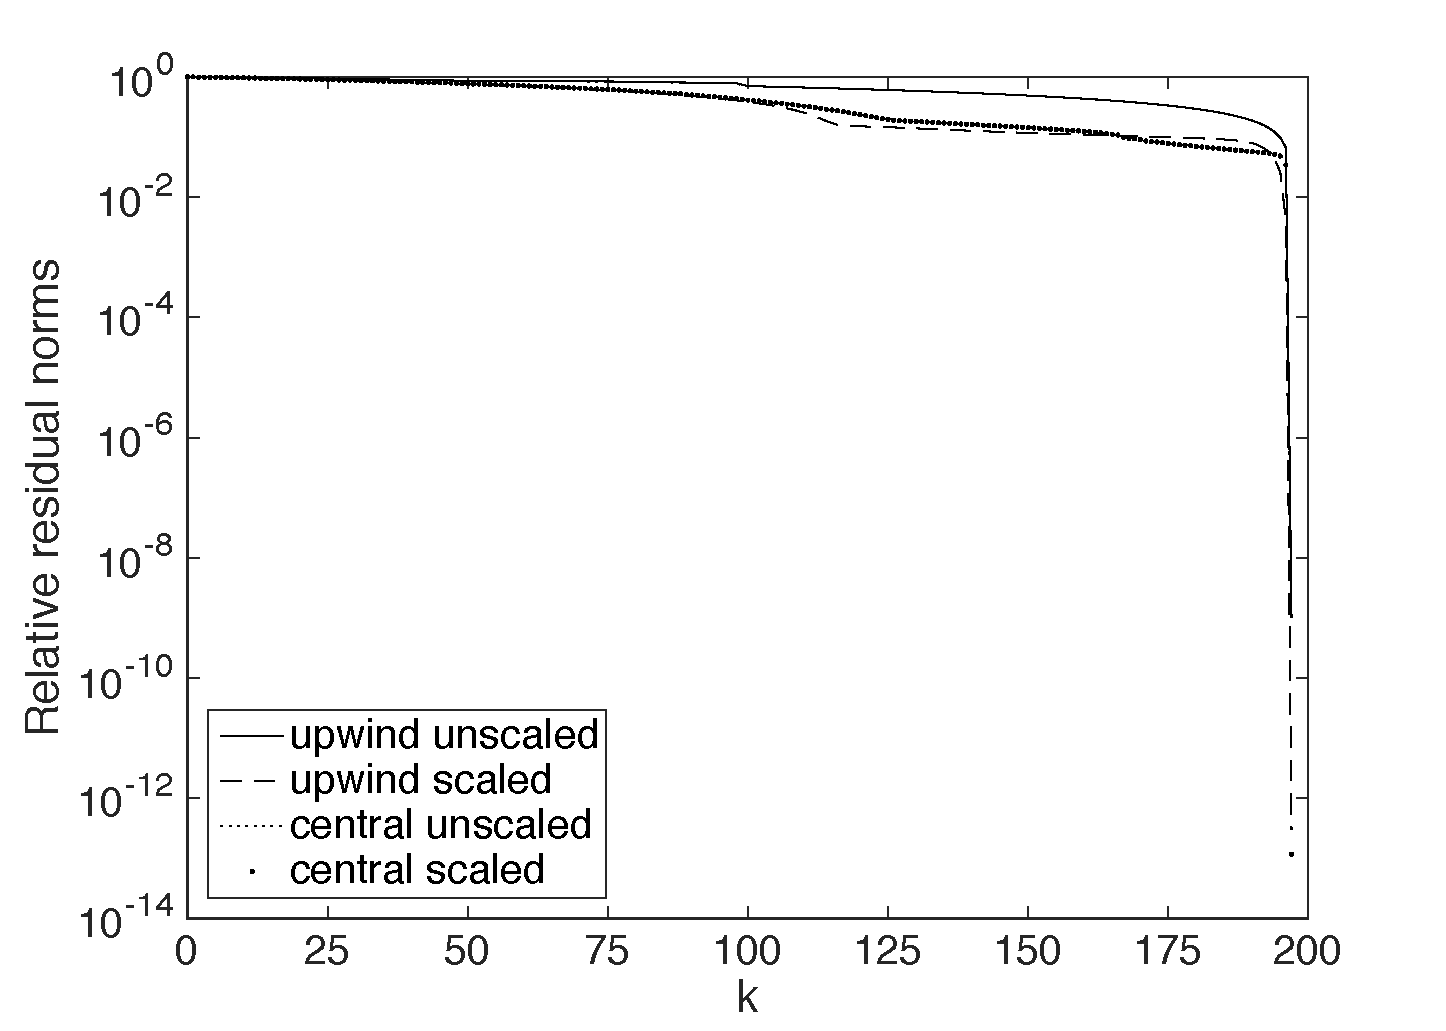
\includegraphics[width=0.95\linewidth]{figures/gmres_4_198}
\caption{GMRES convergence for $\epsilon=10^{-4}$.}\label{fig:back:GMRES.N198.eps4}
\end{minipage}
%
\begin{minipage}[t]{0.48\linewidth}
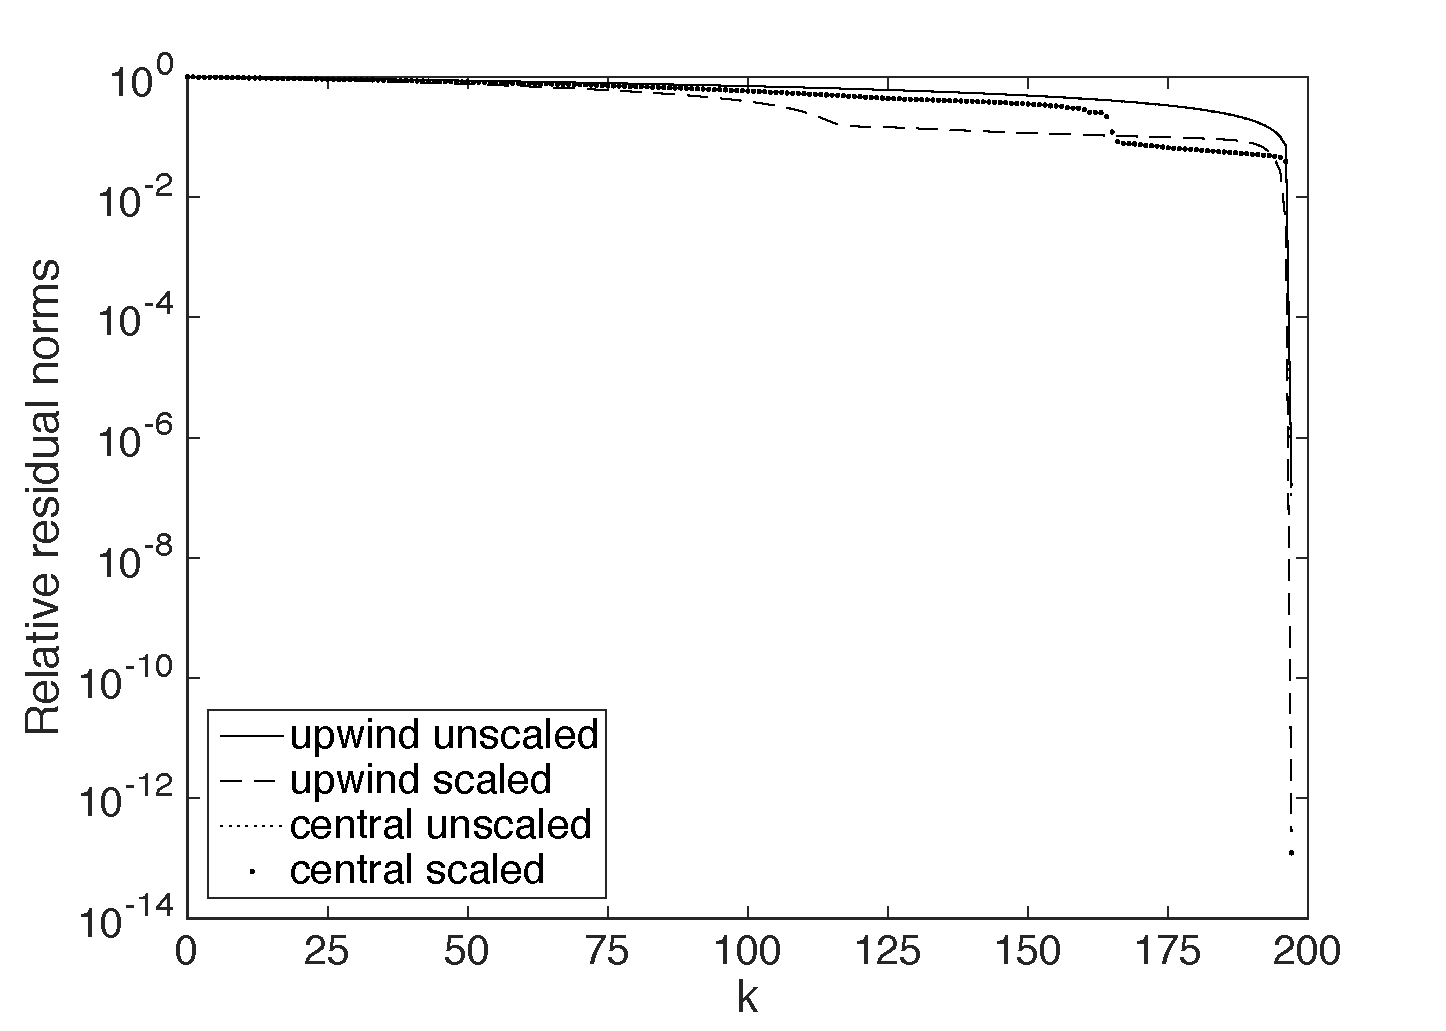
\includegraphics[width=0.95\linewidth]{figures/gmres_6_198}
\caption{GMRES convergence for $\epsilon=10^{-6}$.}\label{fig:back:GMRES.N198.eps6}
\end{minipage}
\end{figure}
%
\begin{figure}
\begin{center}
\begin{minipage}[t]{0.48\linewidth}
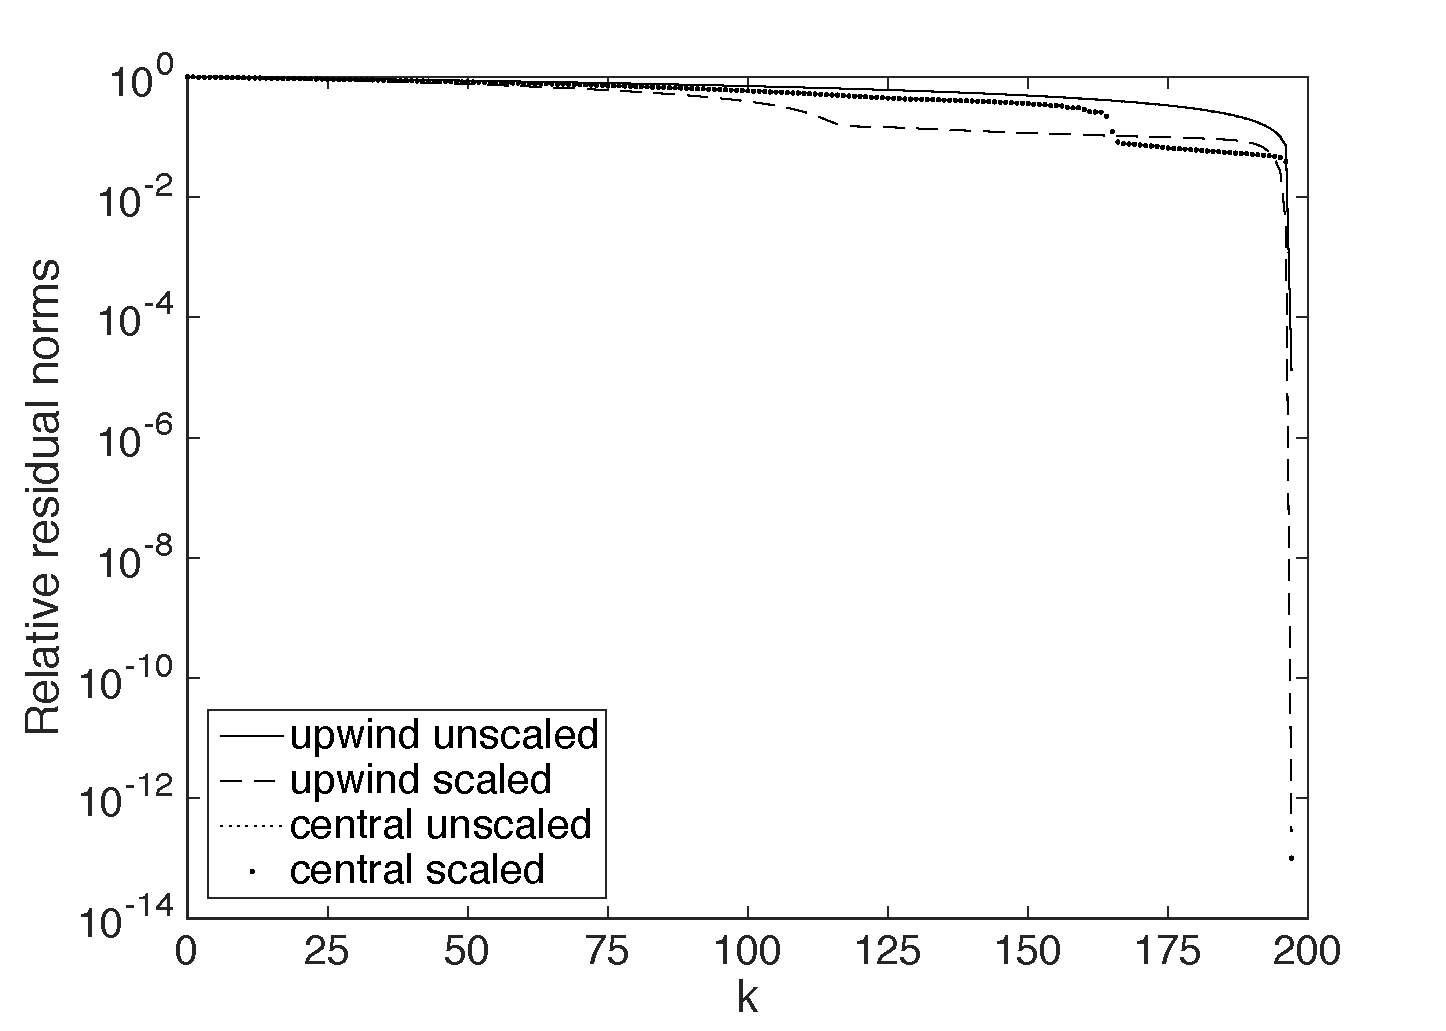
\includegraphics[width=0.95\linewidth]{figures/gmres_8_198}
\caption{GMRES convergence for $\epsilon=10^{-8}$.}\label{fig:back:GMRES.N198.eps4}
\end{minipage}
\end{center}
\end{figure}

\section{Shishkin-Schwarz Preconditioning}
\label{1D:ShishScwarzPrecon}

Based on (\ref{eq:schwarz}), it is clear that the multiplicative Schwarz
method can be seen as a {\em Richardson iteration} for the system
\begin{equation}\label{eq:1D:precond}
(I-T)x=v.
\end{equation}
Furthermore, the iteration scheme (\ref{eq:schwarz}) can be written in the form
\begin{equation*}%\label{eq:schwarz2}
x^{(k+1)}= x^{(k)} + (I-T) (x-x^{(k)}),
\end{equation*}
so that the multiplicative Schwarz method as well as GMRES applied to
(\ref{eq:1D:precond}) obtain their approximations
from the \cred{Krylov subspace $\mathscr{K}_k(I-T,r_0)$.}
Consequently, in terms of the residual norm, GMRES applied to
(\ref{eq:1D:precond}) will always converge faster than the multiplicative Schwarz
method. \cred{Moreover, if one applies GMRES to (\ref{eq:1D:precond}), then the
multiplicative Schwarz method can be seen as a \emph{preconditioner}}
for the GMRES method; see, e.g.,~\cite{KahKamPhi07} where this approach is
taken. The preconditioner $M$ such that $M^{-1}Ax=M^{-1}b$ results in
(\ref{eq:1D:precond}), can formally be written as $M = A (I-T)^{-1}$; see,
e.g.,~\cite[Lemma 2.3]{LanRosSzy91}.

\cred{In general, if a matrix $T$ satisfies $r=\mathrm{rank}(T)$, then for any
initial residual $r_0$ we have
\[\dim \left(\mathscr{K}_k(I-T,r_0)\right) \leq r+1,\]
so that GMRES applied to the system (\ref{eq:1D:precond}) converges to the
solution in at most $r+1$ steps (in exact arithmetic). In the one-dimensional
model problem studied in this paper we have a matrix~$T$ with $r=1$. Thus,
GMRES applied to (\ref{eq:1D:precond}) converges in (at most) two steps
(see Figures~\ref{fig:1D:GMRES.N198.eps4.prec}--\ref{fig:1D:GMRES.N198.eps8.prec}), even when the multiplicative Schwarz
iteration itself converges slowly or diverges, which may happen for the
central difference scheme and $m$ odd. In a generalization of the approach
presented in this paper to two- or three-dimensional problems, and hence more
complicated Shishkin meshes with several transition points, one can possibly
exploit a low rank structure of the iteration matrix as well. }


It is important to point out that, typically, in practical implementations the
local subdomain problems will not be solved exactly. \cred{In the case of
inexact solves} the bounds obtained in this paper and the exact termination of
GMRES in $r+1$ steps will no longer hold.
Nevertheless, the theory for the exact case presented here gives an indication
for the behavior in the inexact case. This is a standard approach in the
context of preconditioning. An example of this framework is given by the
saddle point preconditioners for which GMRES terminates in a few
steps; see~\cite{BenWat08}. In the context of domain decomposition methods, in
particular for Schwarz methods, the concept of inexact subdomain solves was
investigated, e.g., in~\cite[Section~4]{BenFroNabSzy01}.
See also \cite{GanLoiSzy12}, where a similar situation is described for
algebraic optimized Schwarz methods.

\section{Flow-Following Preconditioning}
\label{1D:FlowFollowPrecon}
The name flow following comes from \cite{AndKop96}


\section{Numerical Experiments}
\label{1D:NumericsA}

\begin{figure}
\begin{minipage}[t]{0.49\linewidth}
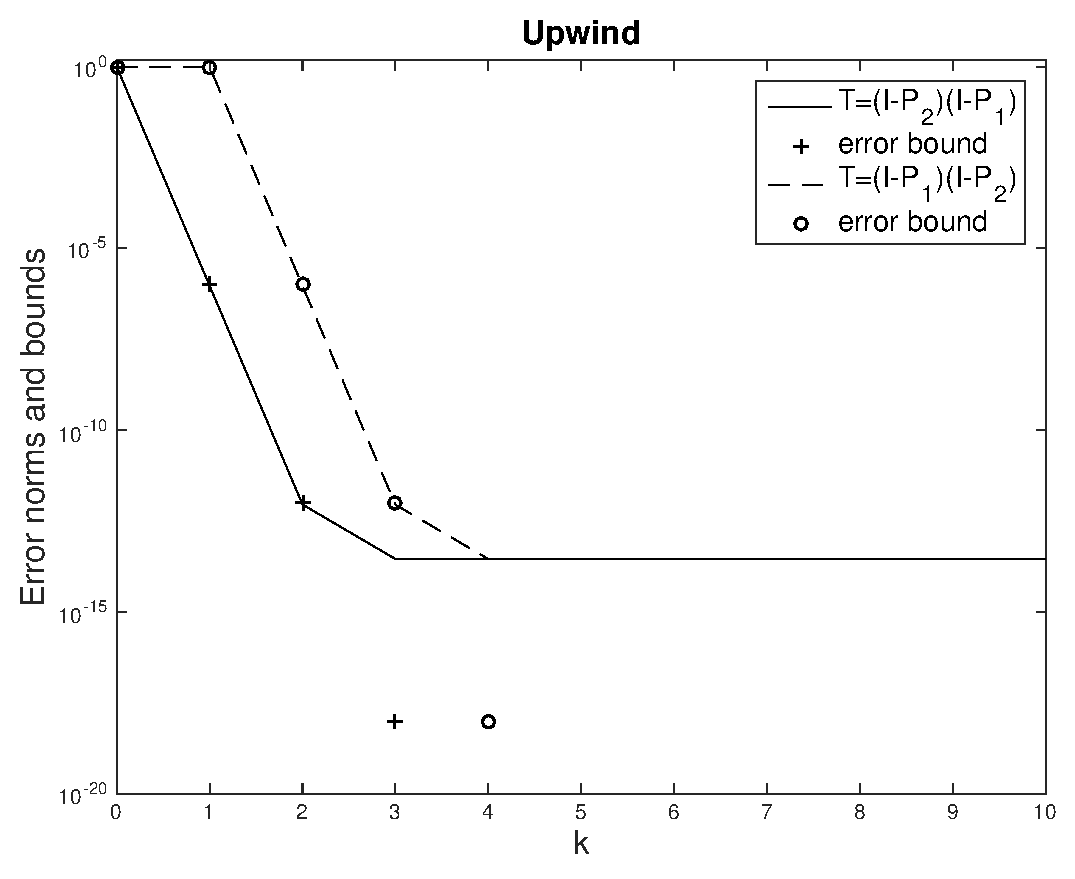
\includegraphics[width=0.95\linewidth]{figures/upwind_8_198}
\end{minipage}
%
\begin{minipage}[t]{0.49\linewidth}
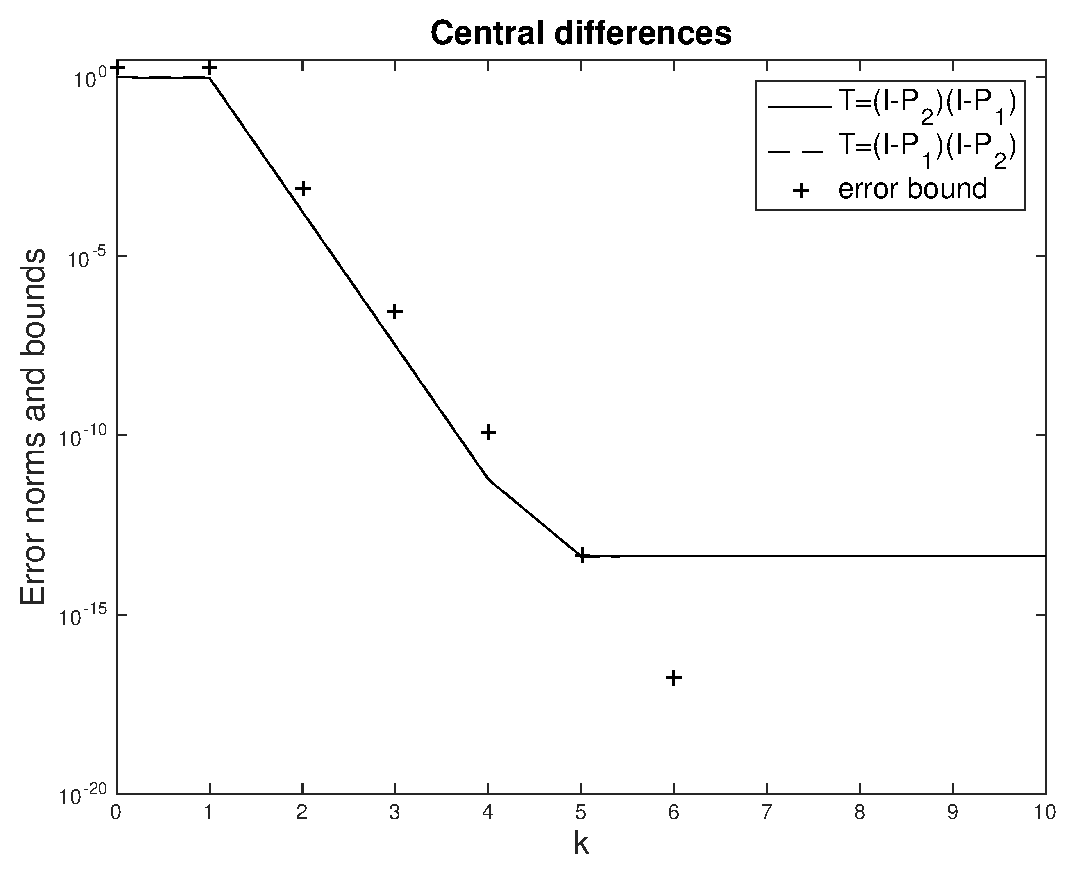
\includegraphics[width=0.95\linewidth]{figures/central_8_198}
\end{minipage}
\caption{Convergence of multiplicative Schwarz and error bounds for
$\epsilon=10^{-8}$, $N=198$.}
%\cblue{Here $|\rho|=9.4\times 10^{-7}<\epsilon(\epsilon+\omega_x H)^{-1}= 9.9 \times 10^{-7}$ for the upwind scheme,
%and $|\rho|=1.8 \times 10^{-4}<2m\epsilon(\epsilon+\omega_x H/2)^{-1}= 3.9 \times 10^{-4}$ for the central differences.}
\label{fig:1D:MSM.N198.eps8}
\end{figure}

\begin{figure}
\begin{minipage}[t]{0.49\linewidth}
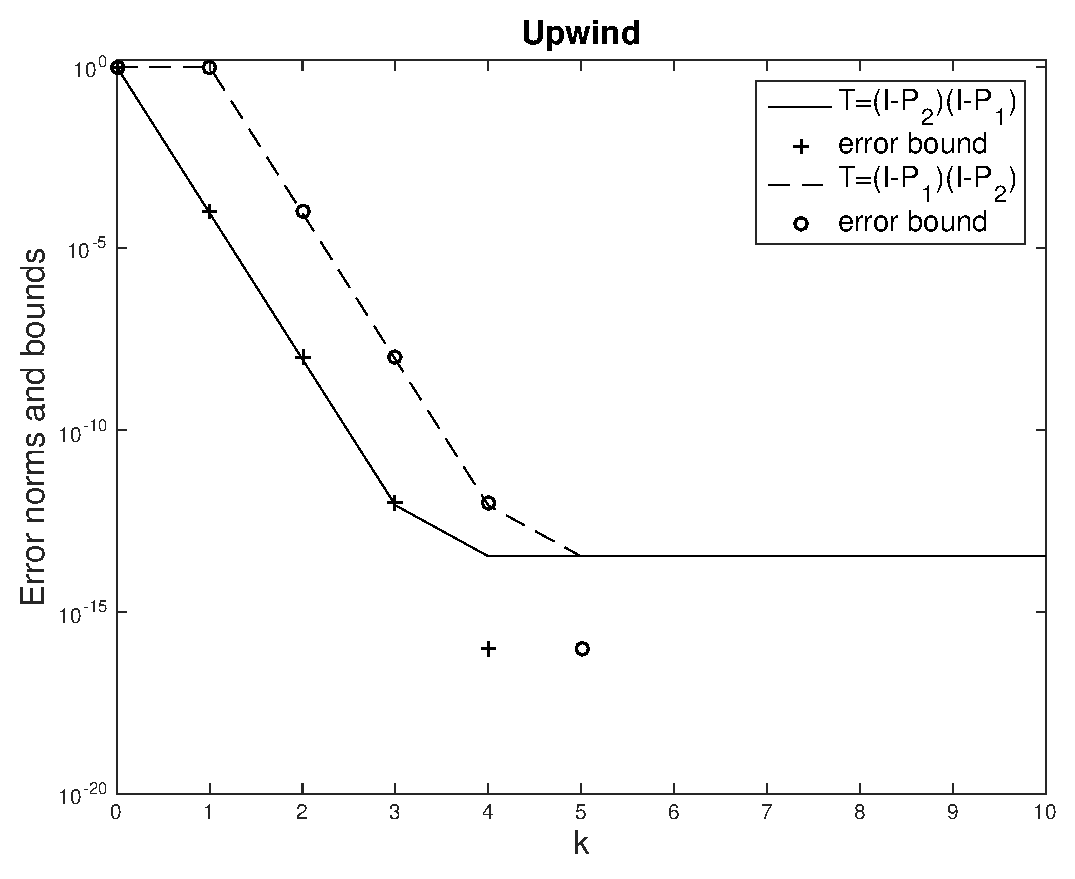
\includegraphics[width=0.95\linewidth]{figures/upwind_6_198}
\end{minipage}
%
\begin{minipage}[t]{0.49\linewidth}
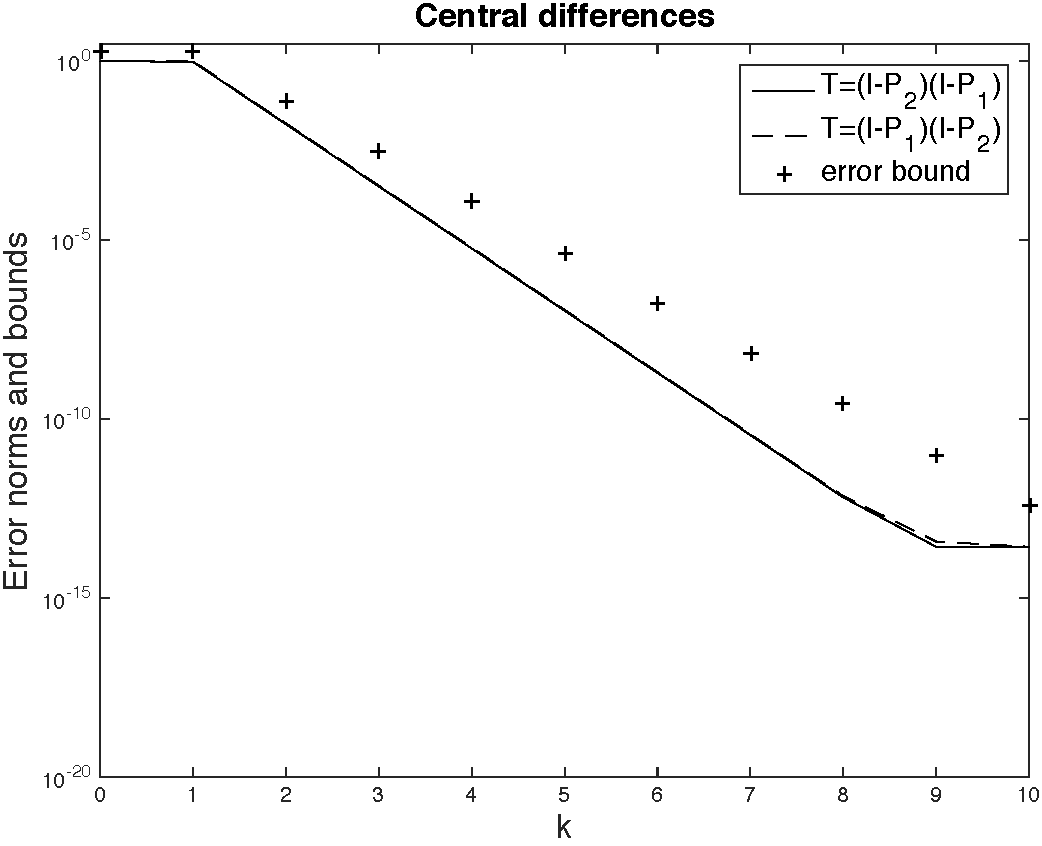
\includegraphics[width=0.95\linewidth]{figures/central_6_198}
\end{minipage}
\caption{Convergence of multiplicative Schwarz and error bounds for
$\epsilon=10^{-6}$, $N=198$. }
%\cblue{Here $|\rho|=9.4\times 10^{-5}<\epsilon(\epsilon+\omega_x H)^{-1}= 9.9 \times 10^{-5}$ for the upwind scheme,
%and $|\rho|=1.8 \times 10^{-2}<2m\epsilon(\epsilon+\omega_x H/2)^{-1}= 3.9 \times 10^{-2}$ for the central differences.}
\label{fig:1D:MSM.N198.eps6}
\end{figure}

\begin{figure}
\begin{minipage}[t]{0.49\linewidth}
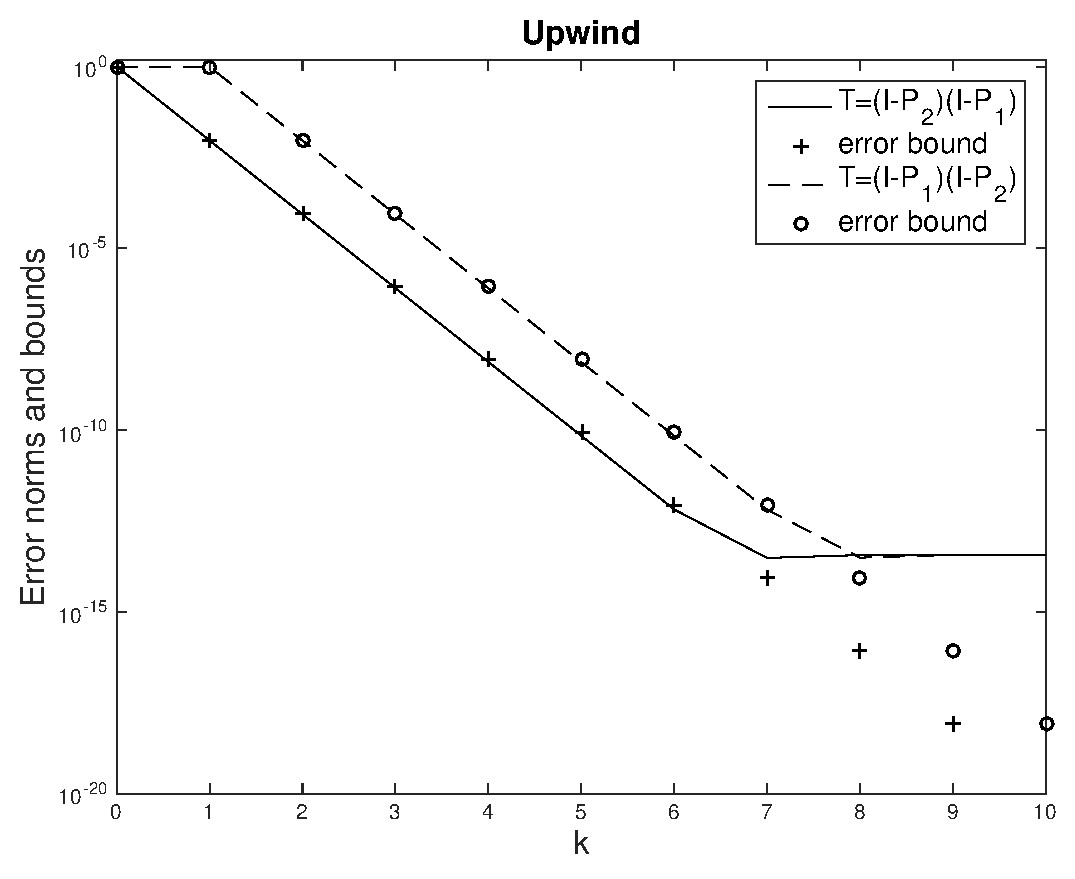
\includegraphics[width=0.95\linewidth]{figures/upwind_4_198}
\end{minipage}
%
\begin{minipage}[t]{0.49\linewidth}
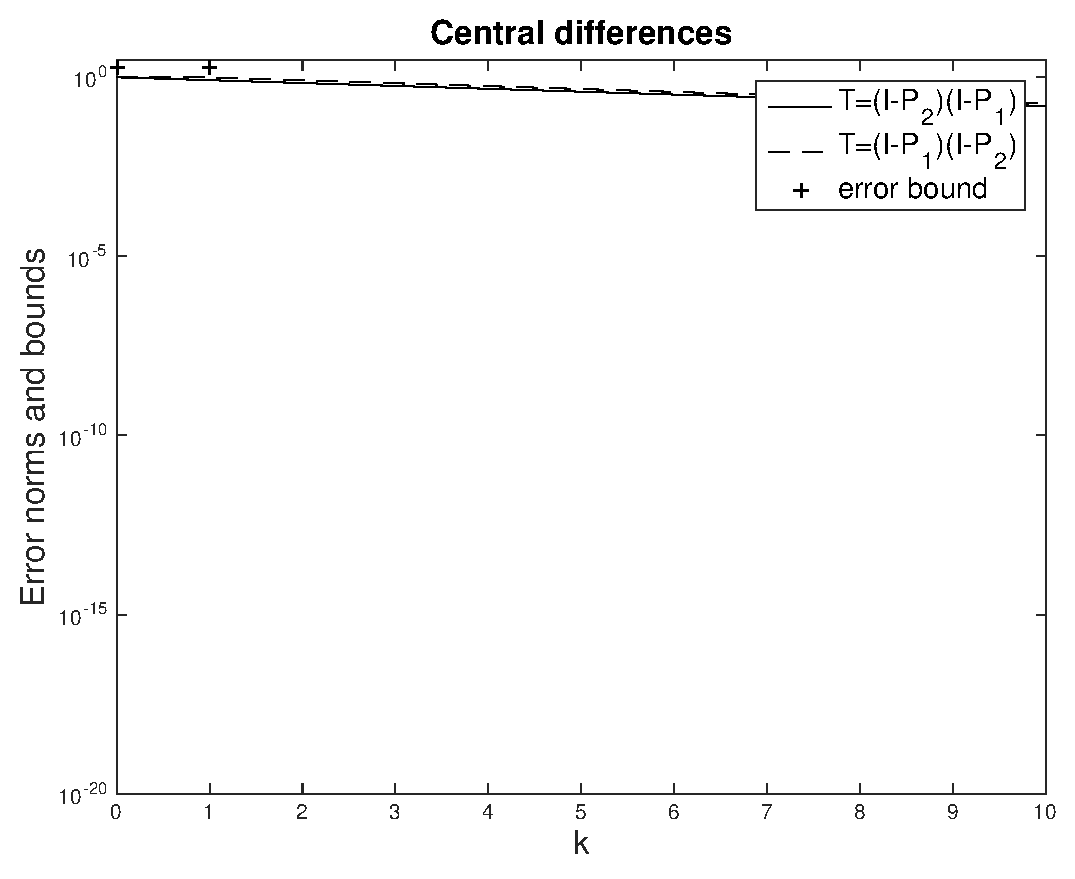
\includegraphics[width=0.95\linewidth]{figures/central_4_198}
\end{minipage}
\caption{Convergence of multiplicative Schwarz and error bounds for
$\epsilon=10^{-4}$, $N=198$. }
%\cblue{Here $|\rho|=9.3\times 10^{-3}<\epsilon(\epsilon+\omega_x H)^{-1}= 9.8 \times 10^{-3}$ for the upwind scheme,
%and $|\rho|=8.3 \times 10^{-1}<2m\epsilon(\epsilon+\omega_x H/2)^{-1}= 3.8$ for the central differences.}
\label{fig:1D:MSM.N198.eps4}
\end{figure}

We now illustrate the convergence behavior of the multiplicative
Schwarz method applied to the Shishkin mesh discretization of the problem
\eqref{eq:1Dbvp} with
%
$$\omega_x=1,\quad \beta=0,\quad f(x)\equiv 1,\quad u_0=u_1=0.$$
%
\cred{The analytic solution of this problem with $\epsilon=0.01$
is shown in Figure~\ref{fig:back:1D_analytic_sol}.

We first consider $N=198$, so that $m=N/2-1=98$ is even.} Recall that the
(unpreconditioned) GMRES method converges very slowly for both types of
discretizations (upwind and central differences); see Figures~\ref{fig:back:GMRES.N198.eps4}--~\ref{fig:back:GMRES.N198.eps4}.

For our experiments we computed $u^N=A^{-1}f^N$ using the backslash operator
in MATLAB.
\cred{(Applying iterative refinement in order to improve the numerical solution
obtained in this way yields virtually the same results, so we do not consider
iterative refinement here.) Using the solution obtained by MATLAB's backslash,
we} computed the error norms of the multiplicative Schwarz method by
$\|e^{(k)}\|_\infty=\|x^{(k+1)}-u^N\|_\infty$ with $x^{(k+1)}$ as in
\eqref{eq:schwarz} (rather than using the update formula
$e^{(k)}=Te^{(k-1)}$). Consequently, the computed error norms
stagnate on the level of the maximal attainable accuracy of the method.
On the other hand, an error bound of the form $|\rho|^k$ for some
$|\rho|<1$ becomes arbitrarily small for $k\rightarrow\infty$.


\begin{figure}
\begin{minipage}[t]{0.49\linewidth}
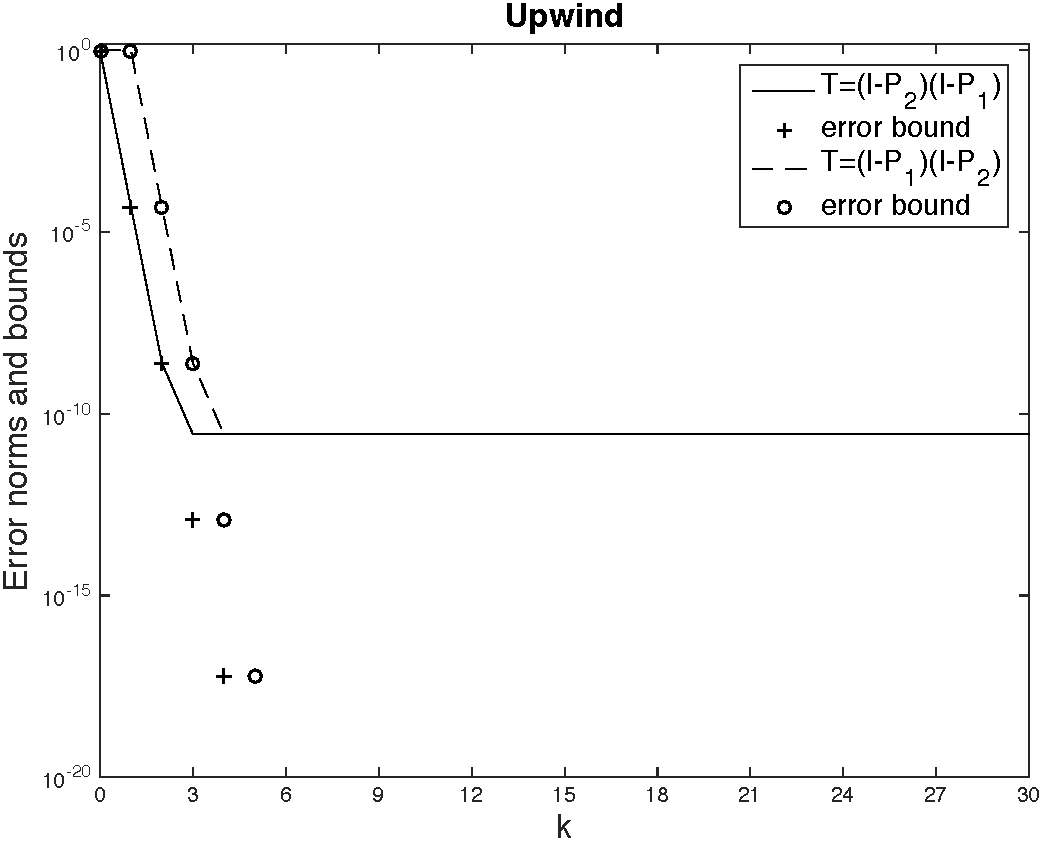
\includegraphics[width=0.95\linewidth]{figures/upwind_8_10002}
\end{minipage}
%
\begin{minipage}[t]{0.49\linewidth}
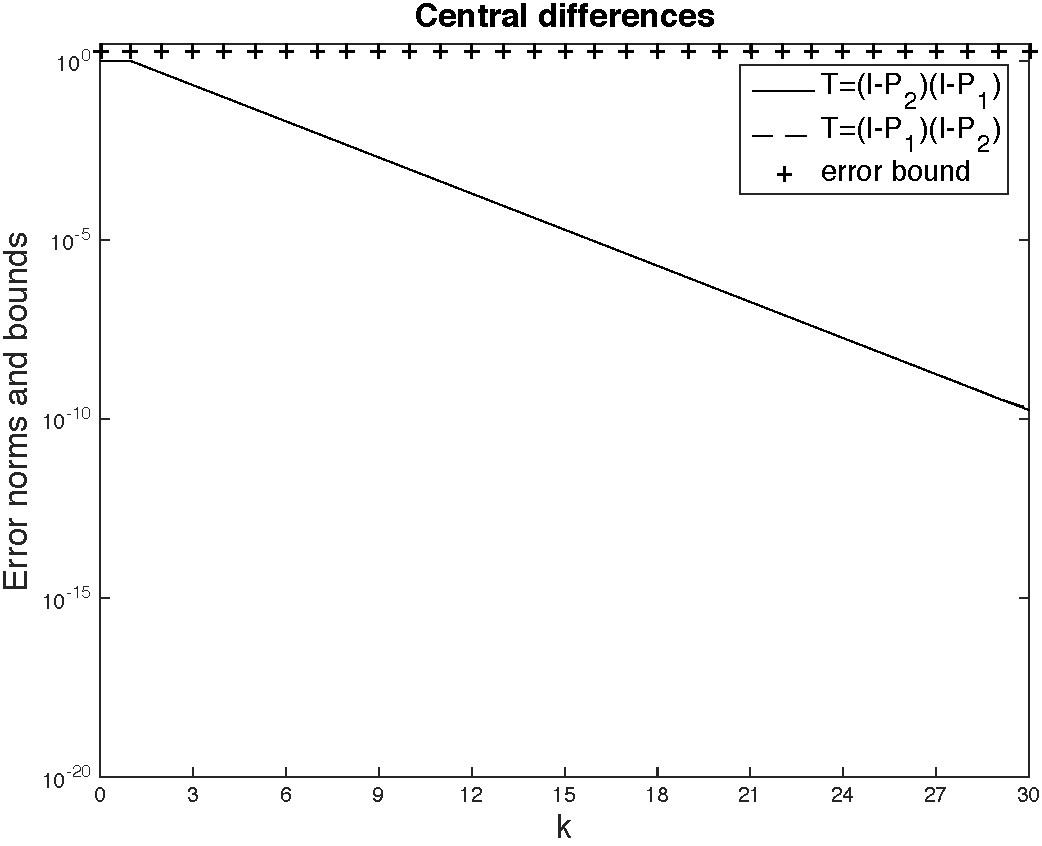
\includegraphics[width=0.95\linewidth]{figures/central_8_10002}
\end{minipage}
\caption{Convergence of multiplicative Schwarz and error bounds for
$\epsilon=10^{-8}$, $N=10002$. }
%\cblue{Here $|\rho|=9.3\times 10^{-3}<\epsilon(\epsilon+\omega_x H)^{-1}= 9.8 \times 10^{-3}$ for the upwind scheme,
%and $|\rho|=8.3 \times 10^{-1}<2m\epsilon(\epsilon+\omega_x H/2)^{-1}= 3.8$ for the central differences.}
\label{fig:1D:MSM.N10002.eps8}
\end{figure}

\begin{figure}
\begin{minipage}[t]{0.49\linewidth}
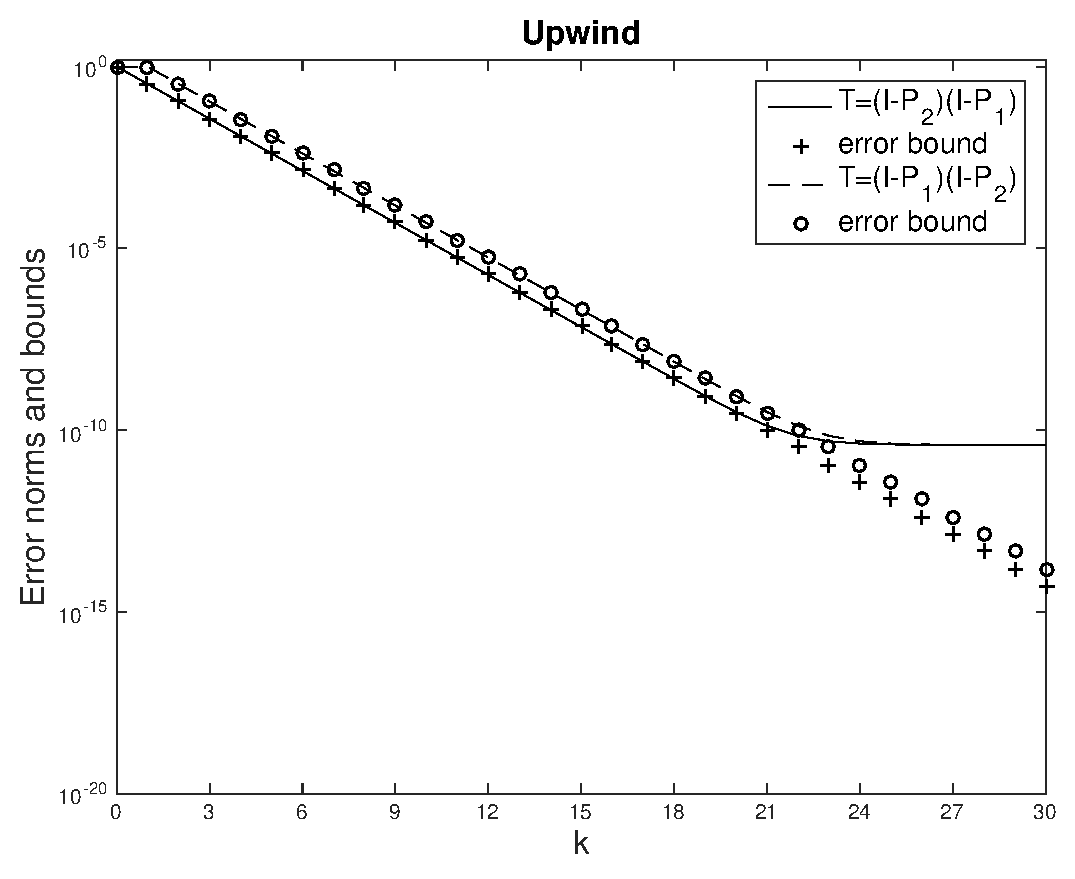
\includegraphics[width=0.95\linewidth]{figures/upwind_4_10002}
\end{minipage}
%
\begin{minipage}[t]{0.49\linewidth}
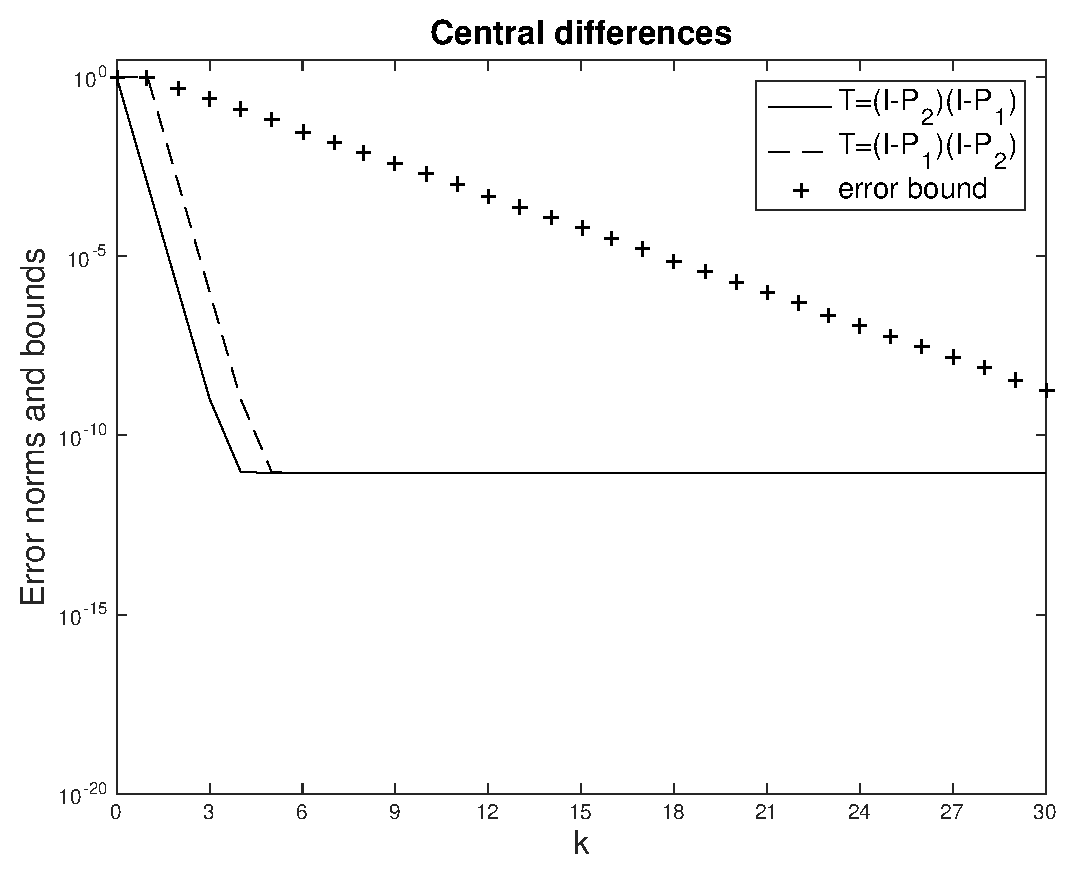
\includegraphics[width=0.95\linewidth]{figures/central_4_10002}
\end{minipage}
\caption{Convergence of multiplicative Schwarz and error bounds for
$\epsilon=10^{-4}$, $N=10002$. }
%\cblue{Here $|\rho|=9.3\times 10^{-3}<\epsilon(\epsilon+\omega_x H)^{-1}= 9.8 \times 10^{-3}$ for the upwind scheme,
%and $|\rho|=8.3 \times 10^{-1}<2m\epsilon(\epsilon+\omega_x H/2)^{-1}= 3.8$ for the central differences.}
\label{fig:1D:MSM.N10002.eps4}
\end{figure}

We start with the upwind discretization. The left parts of Figures~\ref{fig:1D:MSM.N198.eps8}--
\ref{fig:1D:MSM.N10002.eps4} show the error norms
%
$$\frac{\|e^{(k)}\|_\infty}{\|e^{(0)}\|_\infty},\quad  k=0,1,2\dots,$$
%
for the iteration matrices $T=(I-P_1)(I-P_2)$ (solid) and $T=(I-P_1)(I-P_2)$
(dashed) as well as the corresponding upper bounds from
Theorem~\ref{thm:1D:upwind_conv},
for increasing values of $\epsilon$. We observe that the bounds are
quite close to the actual errors. Moreover, in each case the error norm for
the multiplicative Schwarz method with the iteration matrix $T=(I-P_1)(I-P_2)$
almost stagnates in the first step, as predicted by the bound in
Theorem~\ref{thm:1D:upwind_conv}.

On the right parts of Figures~\ref{fig:1D:MSM.N198.eps8}--\ref{fig:1D:MSM.N10002.eps4} we show the
error norms of the multiplicative Schwarz method and the corresponding
convergence bounds from Theorem~\ref{thm:central_conv} for the central
difference scheme.
For our choice of parameters we have $\omega_x H > 2\epsilon$. Note that the
error norms are virtually the same for both iteration matrices. However,
the bounds are not as tight as for the upwind scheme. For fixed $N$ the bounds
become weaker with increasing $\epsilon$, i.e., decreasing convection-
dominance. For our chosen parameters and $\epsilon=10^{-4}$,
giving $\epsilon N^2=\mathscr{O}(1)$, the convergence of the multiplicative
Schwarz method becomes very slow, and the bound~(\ref{eq:1D:bound2}) fails to
predict convergence at all.
The values of $|\rho|$ and the corresponding bounds from
Theorems~\ref{thm:1D:upwind_conv} and \ref{thm:central_conv} are shown in
Table~\ref{t:rho} for the case $N=198$. We observe that the bounds on $|\rho|$
for the upwind scheme are tighter than for the central difference scheme.
\begin{table}[h!]\centering
%\begin{tabular}{rc|c||c|c}
\begin{tabular}{r|c c |c c}
%\cline{2-5}
  & \multicolumn{2}{ c | }{upwind} & \multicolumn{2}{ c }{central differences}\\ \hline
% & \multicolumn{2}{ c|| }{upwind} & \multicolumn{2}{ c }{central differences}\\ \hline
\multicolumn{1}{ c|   }{$\epsilon$}&$|\rho|$~\eqref{eq:1D:rho} & bound~\eqref{eq:1D:bound_upw} & $|\rho|$~\eqref{eq:1D:rho} & bound~\eqref{eq:1D:bound2}\\
%\hline
\multicolumn{1}{ c|  }{$10^{-8}$} & $9.4 \times 10^{-7}$ & $9.9 \times 10^{-7}$ & $1.8 \times 10^{-4}$ & $3.9 \times 10^{-4}$\\
\multicolumn{1}{ c|  }{$10^{-6}$} & $9.4 \times 10^{-5}$ & $9.9 \times 10^{-5}$ & $1.8\times 10^{-2}$ & $3.9\times 10^{-2}$\\
\multicolumn{1}{ c|  }{$10^{-4}$} & $9.3 \times 10^{-3}$ & $9.8 \times 10^{-3}$ & $8.3\times 10^{-1}$ & $3.8\times 10^{0}~~$\\
\end{tabular}
\cred{\caption{Values of $|\rho|$ computed using \eqref{eq:1D:rho} and the
corresponding bounds (\ref{eq:1D:bound_upw}) and (\ref{eq:1D:bound2}) for different
$\epsilon$ and $N=198$.}
\label{t:rho}}
\end{table}

We also run the experiments for a larger value of $N$, namely $N=10002$, to
further \cred{illustrate} our results. We consider the special cases
$\epsilon N^2 \approx 1$ (Figure~\ref{fig:1D:MSM.N10002.eps8})
and $\epsilon N \approx 1$ (Figure~\ref{fig:1D:MSM.N10002.eps4})
which are mainly of theoretical interest. While the bound (\ref{eq:1D:bound_upw})
for the upwind scheme is still tight and descriptive, the
bound~(\ref{eq:1D:bound2}) for the central difference scheme does not predict
convergence well.
Note that the parameters used in Figure 5.5 yield $\omega_x H\approx 1.9959
\times 10^{-4} < 2\epsilon$, and hence the right part of Figure 5.5 shows
error norms and the convergence bound corresponding to the case
$\omega_x H\leq 2\epsilon$ in Theorem~\ref{thm:central_conv}.


\cred{We conclude our numerical experiments by applying GMRES to the linear
algebraic system \emph{preconditioned with multiplicative Schwarz}, i.e., the
linear algebraic system \eqref{eq:1D:precond}, in the case $N=198$. The true
(preconditioned) relative residual norms are shown in
Figures~\ref{fig:1D:GMRES.N198.eps4.prec}--\ref{fig:1D:GMRES.N198.eps8.prec}. In all cases convergence is achieved in two
iterations, which is explained in the next section. These figures are the
counterparts to Figures~\ref{fig:back:GMRES.N198.eps4}--\ref{fig:back:GMRES.N198.eps4}, where GMRES makes little
progress until iteration 198.}

\begin{figure}
\begin{minipage}[t]{0.48\linewidth}
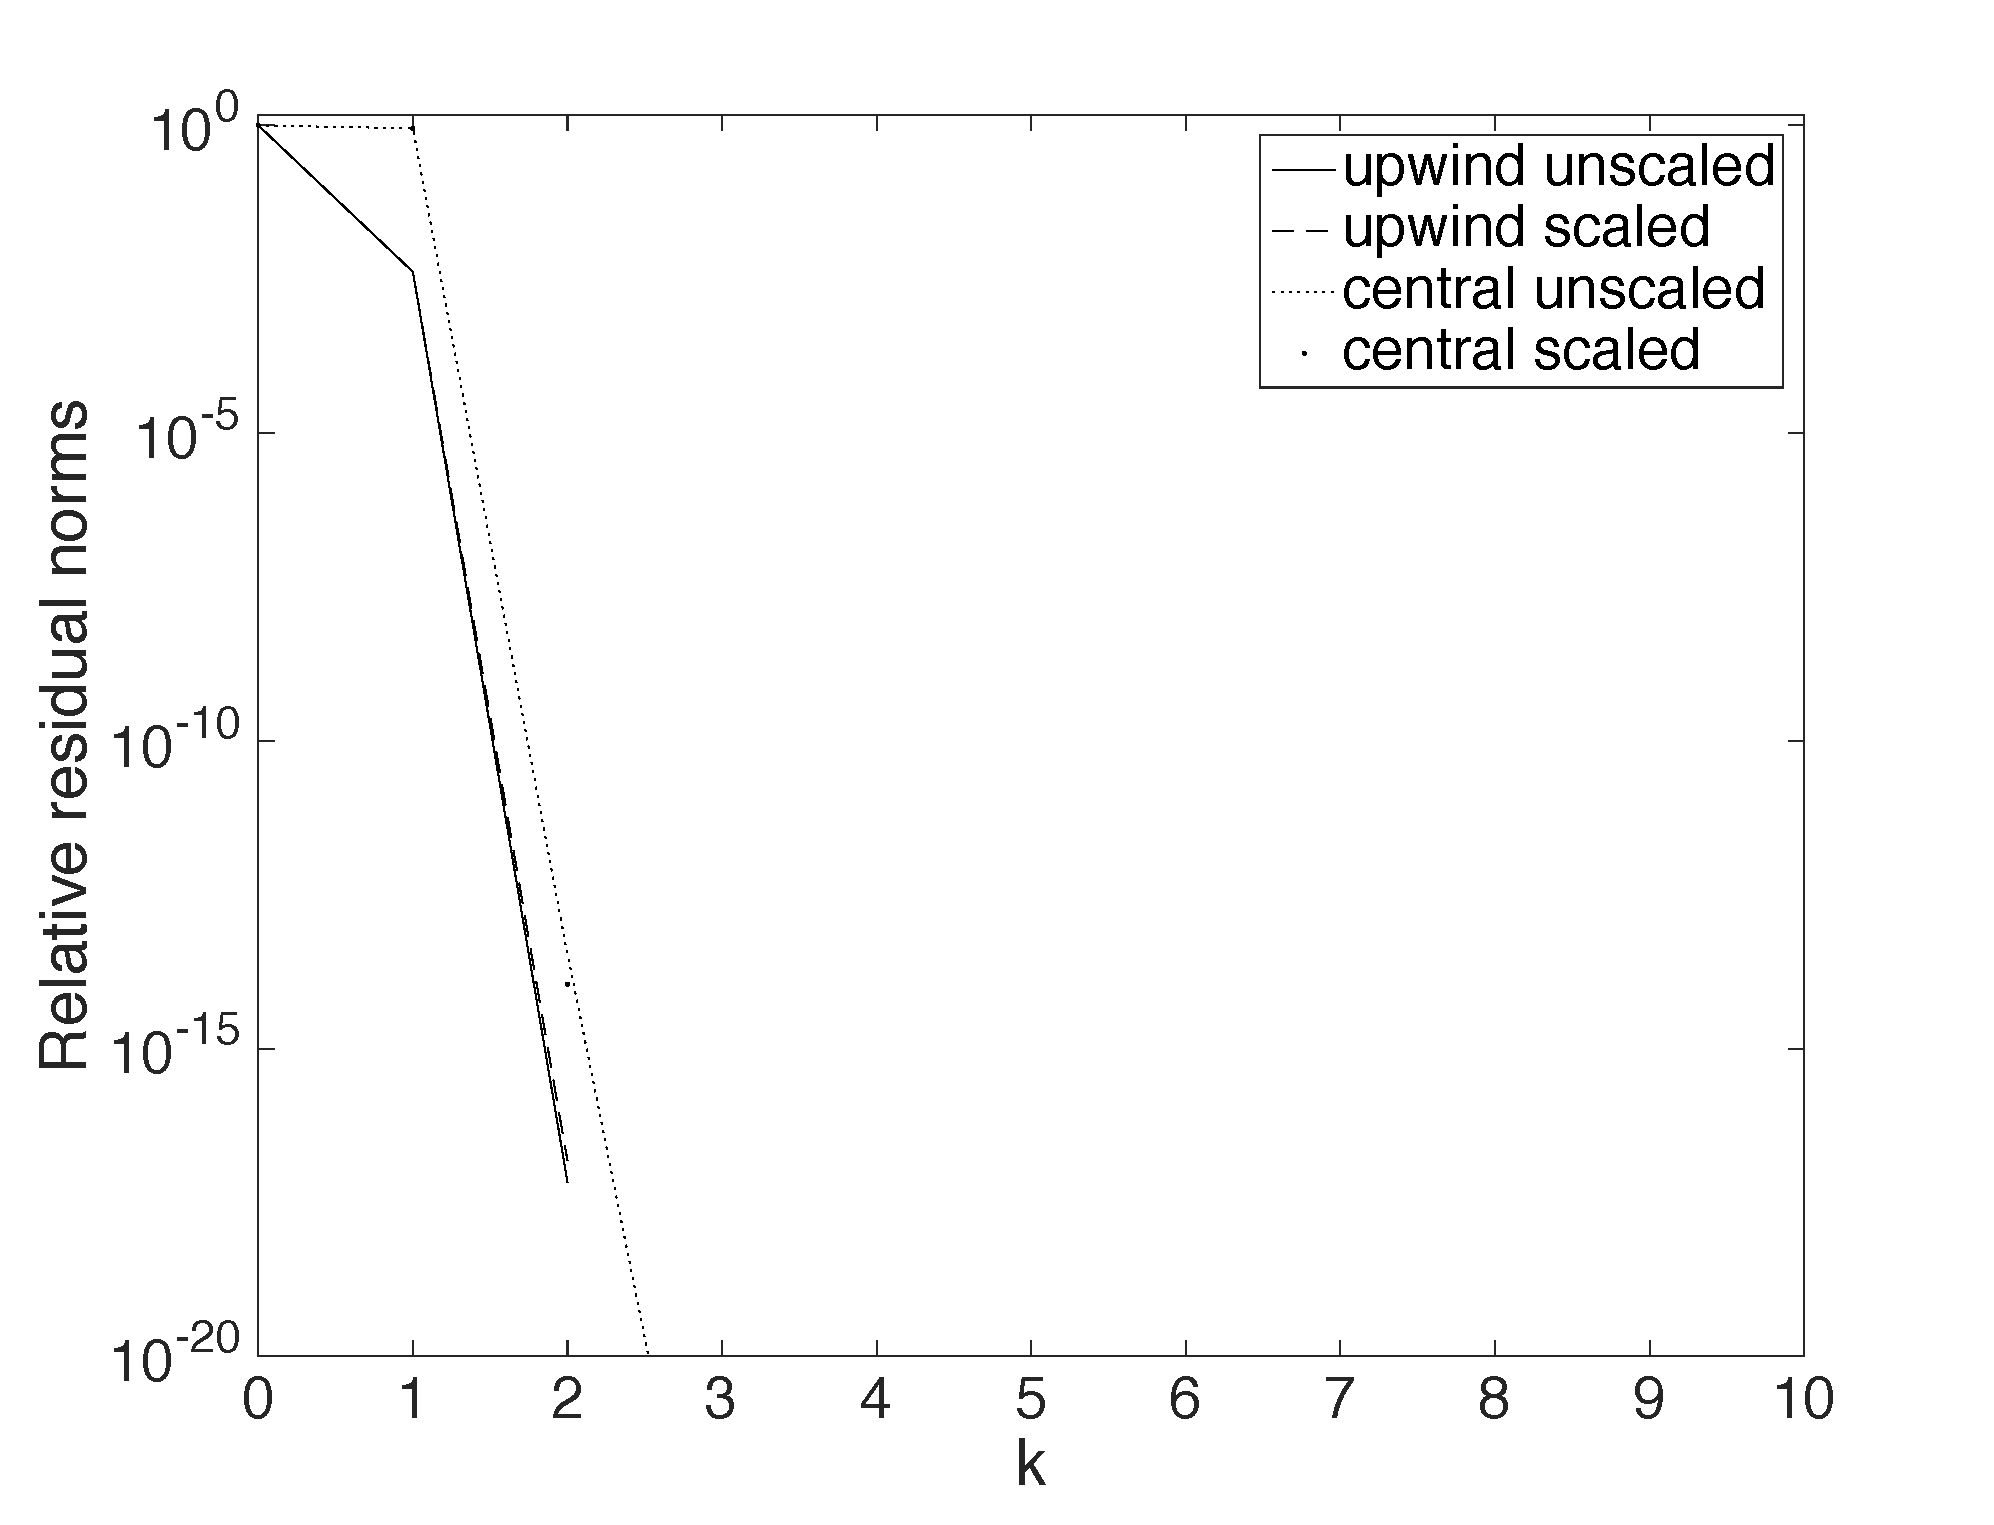
\includegraphics[width=0.98\linewidth]{figures/gmres_4_198_prec.pdf}
\caption{GMRES convergence for $\epsilon=10^{-4}$.}\label{fig:1D:GMRES.N198.eps4.prec}
\end{minipage}
%
\begin{minipage}[t]{0.48\linewidth}
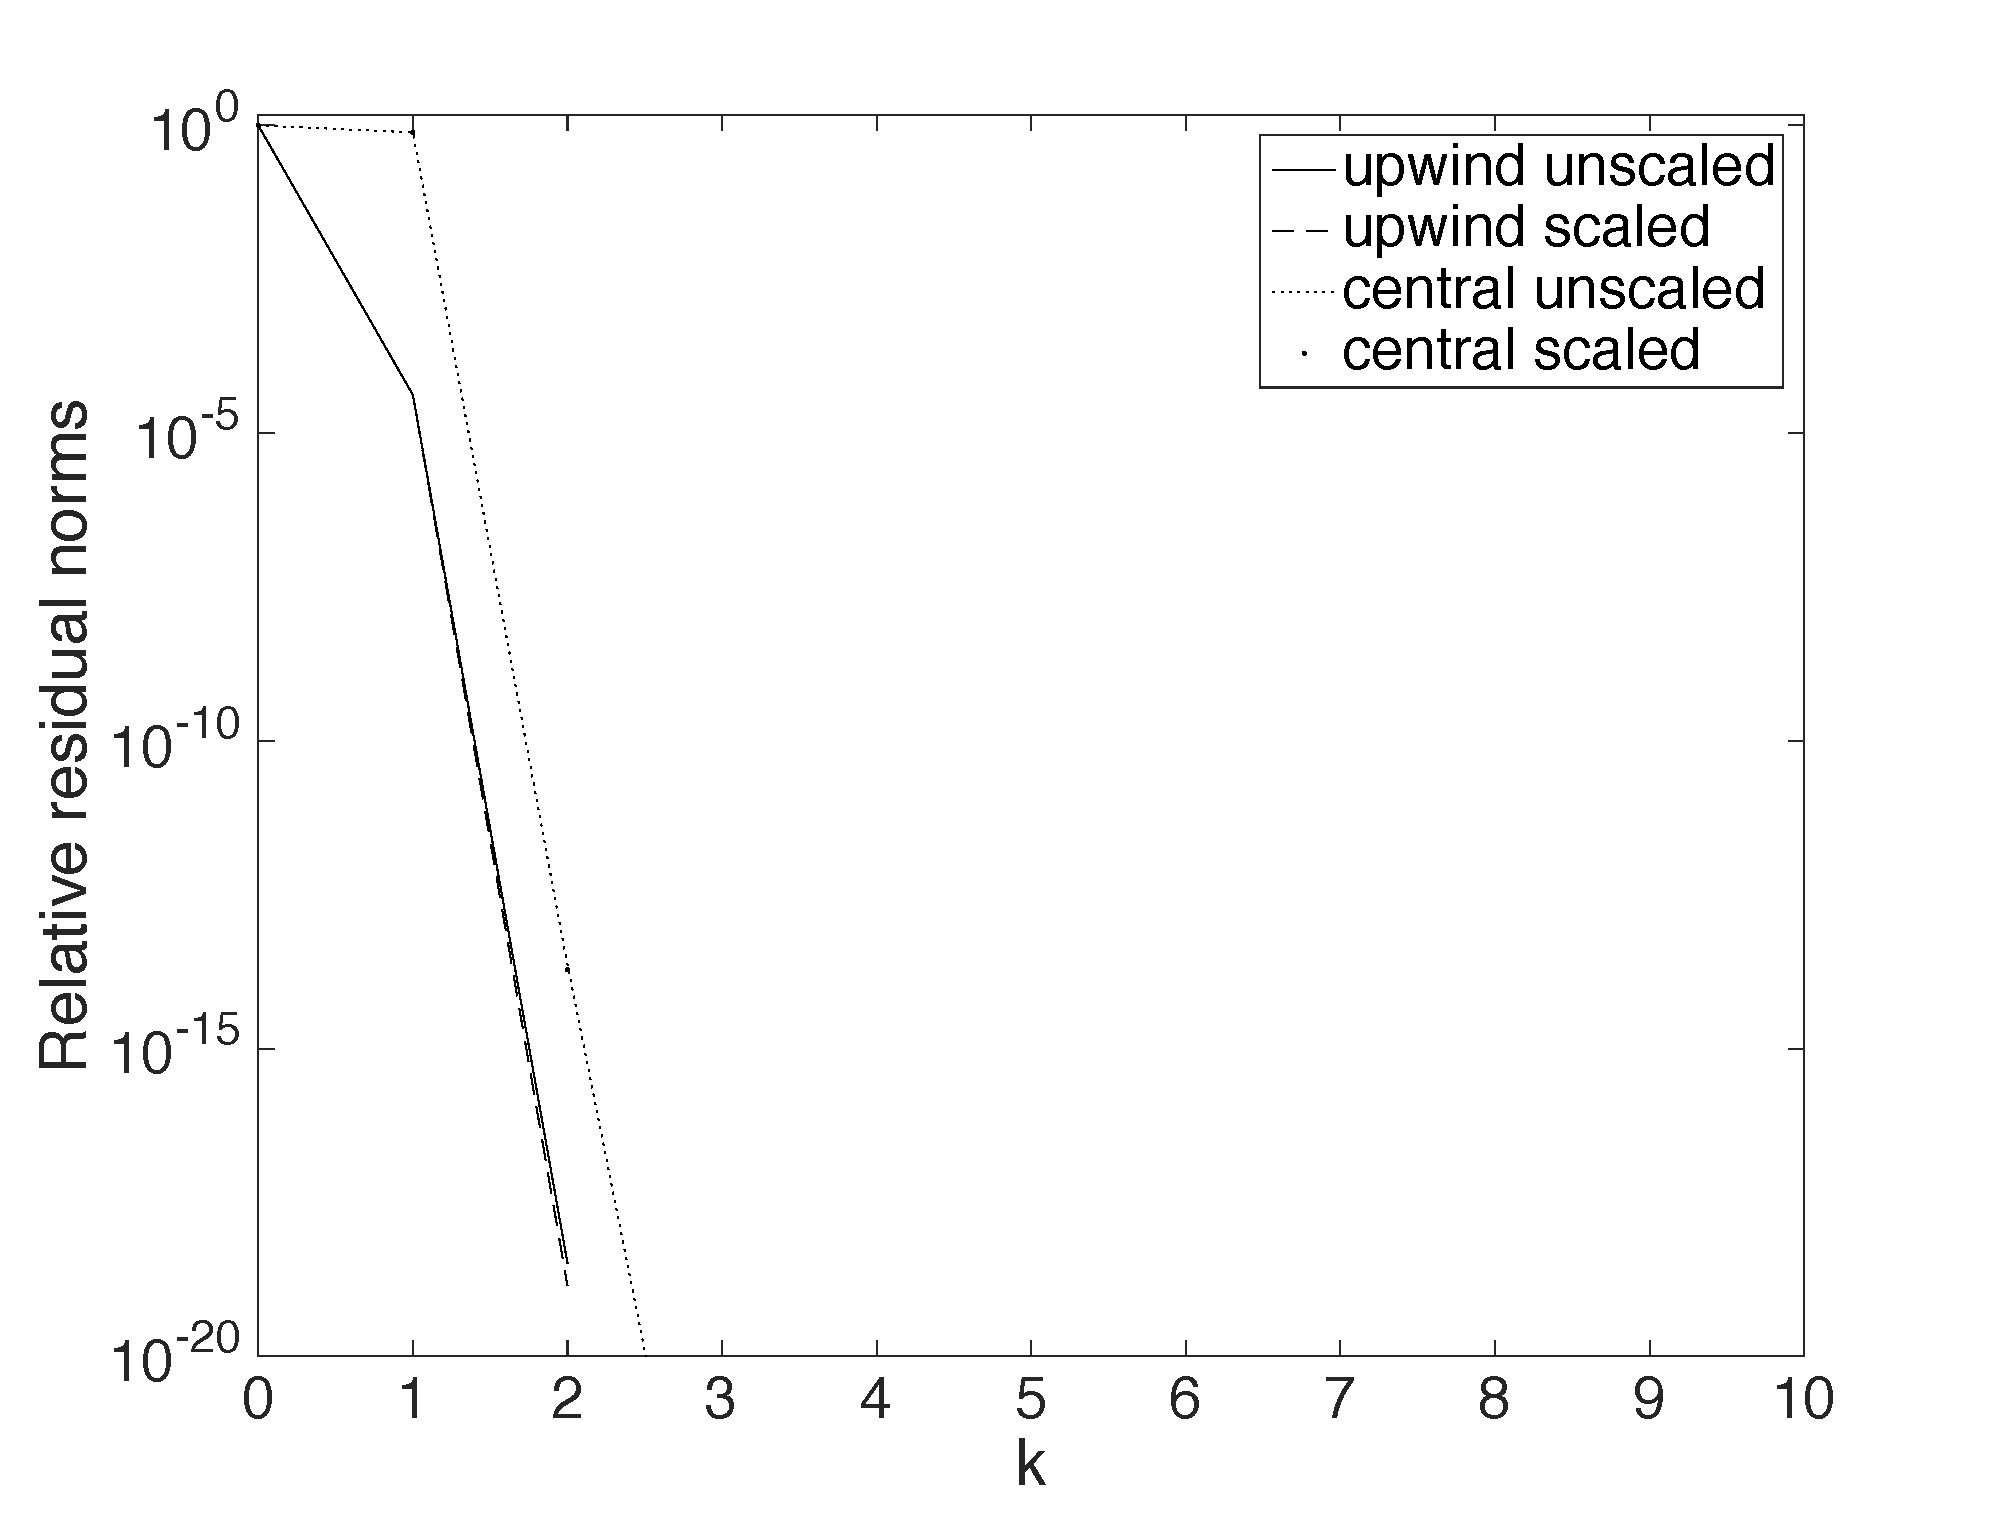
\includegraphics[width=0.98\linewidth]{figures/gmres_6_198_prec.pdf}
\caption{GMRES convergence for $\epsilon=10^{-6}$.}\label{fig:1D:GMRES.N198.eps6.prec}
\end{minipage}
\end{figure}
%
\begin{figure}
\begin{center}
\begin{minipage}[t]{0.48\linewidth}
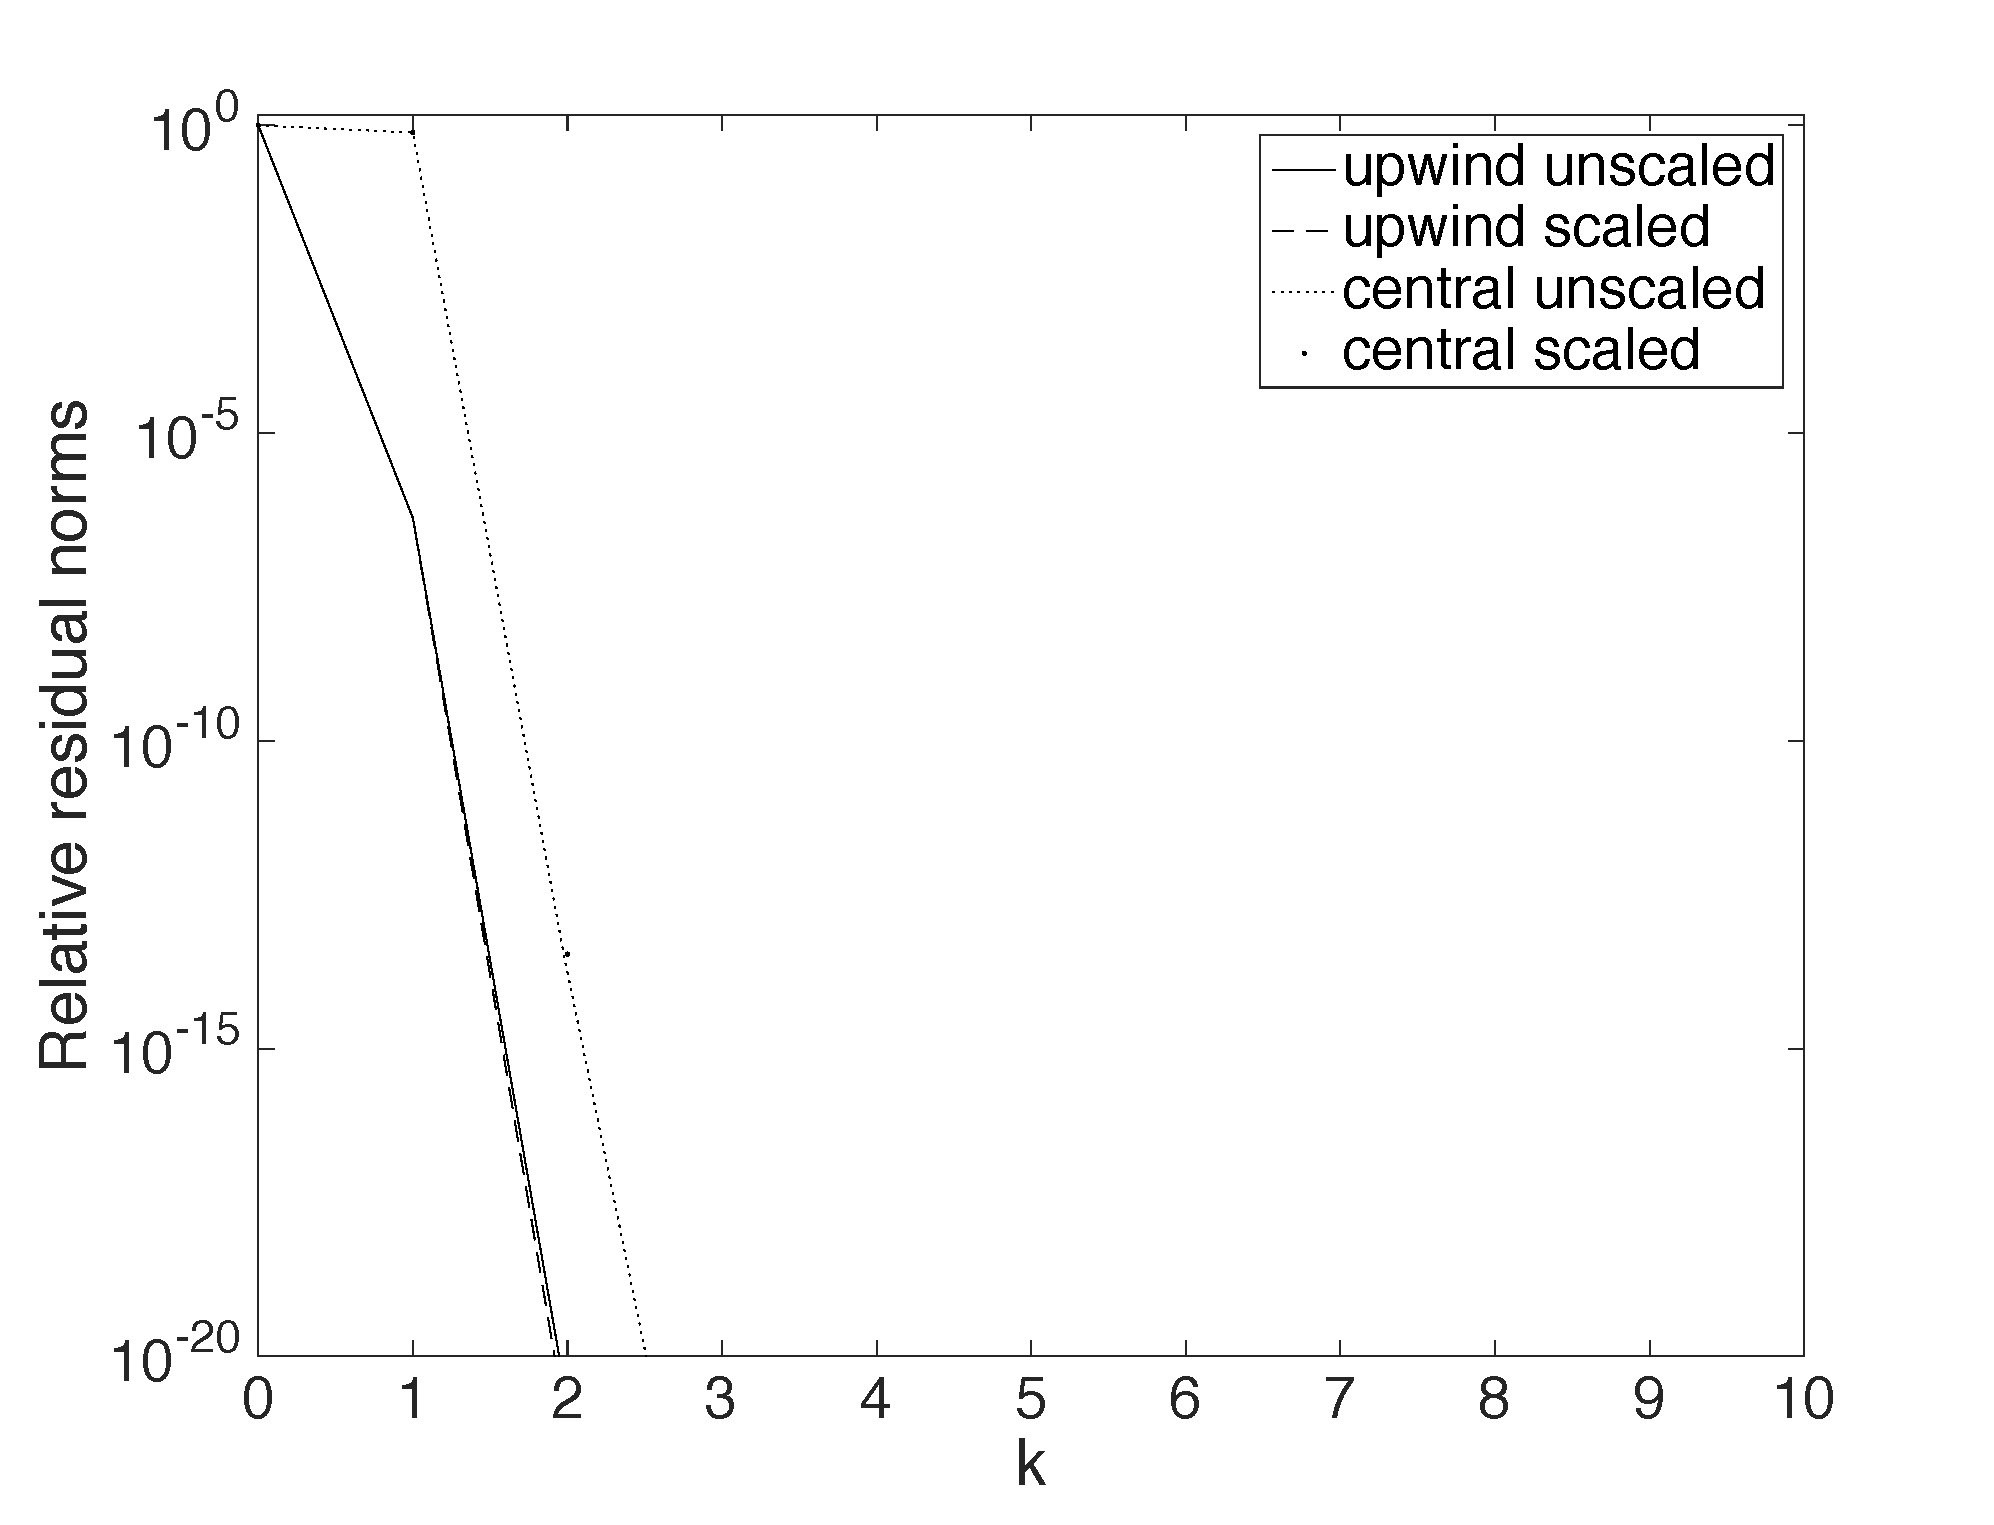
\includegraphics[width=0.98\linewidth]{figures/gmres_8_198_prec.pdf}
\caption{GMRES convergence for $\epsilon=10^{-8}$.}\label{fig:1D:GMRES.N198.eps8.prec}
\end{minipage}
\end{center}
\end{figure}
%
\subsection{Upwind Finite Differences}


\subsection{Central Finite Differences}


%\cred{Finally, we conclude our numerical experiments with an example
%\cblue{for the central differences scheme, showing the behavior of the considered linear solvers in the case %when $m=N/2-1$ is odd. Recall that if $m$ is odd, we are not able to bound the terms which appear in
%the explicit form of $\rho$ (see \eqref{eq:1D:rho}) as in Lemma~\ref{lem:p4}.
%In the experiment we choose $\epsilon=10^{-3}$ and $N=20$ so that $m=9$.
%In the right part of Figure~\ref{fig6} we see that the multiplicative Schwarz method diverges and obviously %$|\rho|>1$. In the right part
%of Figure~\ref{fig6} we apply GMRES to the system preconditioned
%with multiplicative Schwarz.
%
%\begin{figure}
%\begin{minipage}[t]{0.48\linewidth}
%\includegraphics[width=0.98\linewidth]{figures/central_3_20}
%\end{minipage}
%
%\begin{minipage}[t]{0.48\linewidth}
%\includegraphics[width=0.98\linewidth]{figures/gmres_3_20_prec}
%\end{minipage}
%\cblue{\caption{Convergence history of multiplicative Schwarz (left) and GMRES (right) for $\epsilon=10^{-3}$, %$N=20$.}\label{fig6}}
%\end{figure}
%
%As in the case of an even $m$, convergence of GMRES is achieved
%in two iterations. This is not surprising thanks to the low rank structure of the iteration matrix, as we will %explain in detail in the  next section. To check the quality of the solution obtained by the preconditioned %GMRES method we computed the relative distance
%$$
%	\frac{\| \bar{x}-x_2\|}{\|\bar{•}{x}\|},
%$$
%where $x_2$ is the GMRES solution and $\bar{x}$ is the solution computed by the MATLAB's backslash operator. %The resulting relative distance is about $???$, and $\|\bar{x}\| \approx ???$.
% }}



%\begin{figure}
%\begin{minipage}[t]{0.48\linewidth}
%\includegraphics[width=0.98\linewidth]{figures/solutions_1_20}
%%\caption{Convergence of multiplicative Schwarz and error bounds for $\epsilon=10^{-3}$, $N=20$.}
%\end{minipage}
%%
%\begin{minipage}[t]{0.48\linewidth}
%\includegraphics[width=0.98\linewidth]{figures/solutions_2_20}
%%\caption{GMRES convergence for $\epsilon=10^{-3}$.}\label{fig9}
%\end{minipage}
%\cred{\caption{Solution of \eqref{eq:bvp} with $\epsilon=10^{-3}$, $\omega_x=1$, $\beta=0$, $f(x)\equiv 1$, $u_0=u_1=0$, and, $N=20$. }\label{fig8}}
%\end{figure}

%As we can see, even though the multiplicative Schwarz method does not converge in this case providing an unsatisfactory numerical solution, the preconditioned system is solved to a desired accuracy yielding and acceptable numerical solution to the problem. Thus we have shown that the restriction of choosing an even number of points in the local subdomains does not affect the performance of the method used as a preconditioner. We provide the following explanation; since
%$$
%\rho(T)\leq\|T\|\leq\gamma<1,
%$$
%the preconditioned system $M^{-1}A=T=I-M^{-1}N$ will have eigenvalues
%$$
%\lambda(M^{-1}A)\subseteq \left\{ z\in\mathbb{R}: |z|<1+\gamma\right\}.
%$$
%We can therefore expect that the GMRES method converges independently of the number of discretization points used in the method as long as the norm of the iteration matrix is less than one.

\fi % end of if statement regarding content shown



% @article{LieStr03-2,
%  author = {Liesen, J. and Strako\v{s}, Z.},
%  doi = {10.1002/pamm.200310},
%  journal = {Proceedings in Applied Math and Mechanics},
%  pages = {551--552},
%  title = {Slow initial convergence of GMRES for SUPG discretized convection-diffusion problems},
%  url = {http://opus.bath.ac.uk/7150/},
%  volume = {3},
%  year = {2003}
% }
